\chapter{Gravitational waves: coincident and coherent searches with short GRB triggers} % Write in your own chapter title
\label{Chapter Four}

\section{Introduction}
In Chapter \ref{Chapter Two} we have outlined the importance of searches for GW triggered by short GRBs whereas in Chapter \ref{Chapter Three} we have described a theoretical background of the analysis techniques used to search for CBC events, in general. These methods have been implemented in two different search \emph{``pipelines''} (coincident and coherent) that have been built for the specific role of searching for CBC events in association with short hard GRBs. ``Pipeline'' refers here to the ensemble of data processing stages that are built to implement the theoretical concepts described in Chapter \ref{Chapter Three}; a pipeline takes the GW detectors' data as input and outputs a list of possible detection events; based on the significance of these events, either a GW detection statement is made, or exclusion distances are computed. 

I used and contributed to the development of both the coincident and coherent pipelines and I will present the workflow, the usage and the search results of these pipelines by means of two examples: a search for CBC events associated with GRB070429B -- in the case of the coincident search during S5/VSR1 and GRB090831A -- in the case of the coherent search during S6/VSR2 and 3. To place these example searches into context, I will also briefly present the search results for GW associated with short GRBs both during S5/VSR1 and S6/VSR2 and 3 science runs.

\section{Coincident triggered search}
\label{coincident_GRB}

Searches for GW associated with short hard gamma-ray bursts have been completed over the last two LIGO and Virgo science runs, see Table \ref{tab:sciencetimes} for the exact dates of these runs, consult \cite{Abadie:2010uf} for results in S5/VSR1 and \cite{lvc:s6grb} for results in S6/VSR23. During S5/VSR1, 22 short hard GRBs observed by \emph{Swift} have been analyzed whereas during S6/VSR2 and 3, 16 GRBs observed by \emph{Swift} and an additional 10 observed by Fermi--GBM have been analyzed. The S5/VSR1 GRBs have been analyzed using the coincident pipeline, described in this section with the help of an example GRB. The S6/VSR2 and 3 GRBs have been analyzed using the coherent pipeline described in the next section, again with the help of an example GRB.

\begin{table}[tp!]
\center
%\begin{ruledtabular}
\begin{tabular}{c | c | c}
\hline
\hline
Science run & Start time & End time \\
\hline
\hline
LIGO -- S5 & 4 November 2005 & 30 September 2007 \\
\hline
Virgo -- VSR1 & 18 May 2007 & 30 September 2007 \\
\hline
LIGO -- S6 & July 7 2009 & October 20 2010 \\
\hline
Virgo -- VSR2 & July 7 2009 & January 11 2010 \\
\hline
Virgo -- VSR3 & August 11 2010 & October 20 2010 \\
\hline
\hline
\end{tabular}
%\end{ruledtabular}
\caption[Duration of LIGO and Virgo science times.]
{The dates of LIGO and Virgo science run times for S5/VSR1 and S6/VSR2 and 3.}
\label{tab:sciencetimes}
\end{table}

Both the coincident and coherent triggered searches use the time and the sky position of the GRB (provided through astronomical observations using the GRB missions and publicly available in NASA's Gamma-ray Circular Notes or GCN, see \cite{gcns}) and uses this information to limit the search to a small time interval and a narrow positional sky error region. The search utilizes the ``coincidence'' technique in which data from all of the detectors is analyzed separately, before looking for events which are coincident between detectors. The coincident triggered search implementation described here is used to search for \ac{CBC} systems whose total masses lie between 2 and 35 $M_{\odot}$ with a minimum component mass of 1 $M_{\odot}$. This choice is motivated by the accepted theory that short GRBs originate from either NS--NS or NS--BH binary coalescences with typical NS masses of 1.4 $M_{\odot}$ and BH masses of 10 $M_{\odot}$ \cite{Abadie:2010uf}. During both S5/VSR1 and S6/VSR2 and 3 an ``ihope'' all--sky--all--time search was carried out as well. The infrastructure the triggered search uses is very similar to the ``ihope'' search described in \cite{Abbott:2009qj} with the exception that the search is done on a much reduced area of the sky and uses a much smaller analysis time around the GRB, thus increasing the sensitivity (see Section \ref{sens_imprv} for a sensitivity comparison between the all--sky, all--time search using ``ihope'' and the GRB triggered search).

The main analysis steps (pipeline workflow) are as follows: data around the time of a short GRB is divided into one ``foreground'' region (containing the GRB event time and where we expect the GW signal to be found) and two ``background'' regions on either side of the ``foreground'' (where we expect no GW signal associated with the GRB). Data from individual operational GW detectors is matched--filtered through detector--specific template banks and using detector--specific PSDs -- the result will be a time--ordered list of events for each detector. Next, the pipeline looks for coincident events within this list (in time and recovered template masses) from all the detectors and applies the $\chi^2$ test on the new coincidences to filter out ``glitches''. The surviving events are collected and a ``detection statistic'' is computed for each, using the match--filter SNR and $\chi^2$ values. Simulated signals are injected in the ``background'' data stretch to test and compute the pipeline's efficiency of signal recovering. Using this efficiency and the ``detection statistic'' of the loudest events, we compute a probability that the loudest ``foreground'' event does or does not belong to the ``background'' statistical sample. In other words, if the event is a signal or noise. In the next sections, we will detail each of these analysis steps and provide the appropriate search results.

\subsection{GRB070429B -- overview}
\label{grb070429boverview}

GRB070429B (GRBlog entry \cite{070429b}) was a short hard gamma-ray burst that was observed on April 29, 2007 at 03:09:04 UTC by the \emph{Swift}/XRT/UVOT satellite. Its characteristic $T_{90}$ duration was 0.5 s and its sky location was right ascension RA=328.02 $\deg$ and declination dec=-38.84 $\deg$. The GRB has a secure host association from a faint sub--arcsecond (position within the UVOT error circle) of an optical afterglow and the host galaxy appears to be a red galaxy \cite{Cenko:2008vt} at redshift $z$=0.904 (luminosity distance of $\approx$4 Gpc). Although this burst has an associated redshift with a corresponding luminosity distance much larger than the typical GW detector range during S5/VSR1 (see Chapter \ref{Chapter Three}), we still performed a GW search since there is a degree of uncertainty in measuring short burst redshifts (see Chapter \ref{Chapter Two} for a reference on assigning redshifts and luminosity distances to short GRB). 

LIGO's operational detectors at the time of the burst were Hanford H1 and Livingston L1. The antenna factors $F = \sqrt{F_{\times}^2+F_+^2}$ for H1 and L1 are 0.99 and 0.93 respectively giving an overall antenna factor of 0.96, revealing an almost overhead position with respect to the H1L1 plane. The astronomical and GW detector data summarizing the characteristics of GRB070429B is presented in Table \ref{Table_grb070429b}.

\begin{table}[ht]
 \begin{tabular}{|l|l|l|l|l|l|}
 \hline
 \hline
 GPS & Date & redshift & $T_{90}$ (s) & RA ($\deg$) & dec($\deg$) \\
 \hline
 861851358 & Apr 29, 2007, 03:09:04 UTC & 0.904 & 0.5 & 328.02 & -38.84 \\
 \hline
 \hline
 \end{tabular}
 \caption{Astronomical and GW detector data for GRB070429B. GRB070429B is a very short gamma-ray burst with $T_{90}$ duration of only 0.5s. The GRB was observed almost overhead by the GW detectors (H1 and L1, with an RMS antenna factor of 0.96). The confirmed redshift of the burst places it at a distance of $\approx$4 Gpc.}
 \label{Table_grb070429b}
\end{table}

\subsection{Data Segments and PSD generation}
\label{grb070429bsegments}

The binary coalescence model of short GRB formation predicts that the time delay between the arrival of a gravitational wave and the arrival of the subsequent gamma-ray burst is a few seconds, see Chapter \ref{Chapter Two}, section ~\ref{SHBmodel}. The gamma-ray burst arrival time is called the \emph{GRB trigger time} and, in this case, it is provided by the \emph{Swift} satellite. We search for gravitational wave signals within an \emph{``on--source''} segment of [-5, +1) s. around the GRB trigger time; this time window should theoretically account for all the the SHB model--dependent uncertainties as well as for the gamma-ray detector's instrumental timing uncertainties.

Since we rely on the assumption that a gravitational wave associated with a GRB should only be detected in the on--source segment, we use off--source \emph{trials} (324, each trial with the length of the on--source, 6 s long) that do not intersect the on--source, to estimate the distribution of \emph{background} due to the accidental coincidences of noise events. We also re--analyze the off--source trials with simulated signals injected in the data to test the response of the search to GW signals; these we call injection trials. To prevent accidental bias in the background estimation due to a potential loud and prolonged signal in the on--source, the off--source segments are padded with 48 s long redundant \emph{buffer} segments on each side of the on--source, the length of these reflecting the longest duration of a matched--filtering waveform. Finally, we discard 72 s of data subject to filter transients on both ends of the off--source region. Taking all these requirements into consideration, the minimum analyzable time \emph{required} for the GW data stretch was $T_{\mathrm{analysis}}=$2190 s and we require that GW detectors should be in continuous science mode for this time, as the character of the background can change between science mode stretches. The data segments are shown in Figure ~\ref{grbsegments}. As we can see the GW detectors with available segments to meet these criteria are H1, H2, G1 and L1. For the S5/VSR1 coincident GRB analysis, the two most sensitive detectors per GRB analysis were used to provide the data; in the case of GRB070429B the two most sensitive detectors were Hanford H1 and Livingston L1.

Both the H1 and L1 strain data were sampled at 16384 Hz. This frequency is actually too high since the highest frequency in each of the matched--filter waveforms is $\approx$2 kHz. To ease computational requirements, the time series is down-sampled to 4096 Hz prior to analysis and a low--pass filter is applied with a cut--off frequency at 2048 Hz. At the lower end of the frequency spectrum, the data is affected by seismic noise (see Chapter \ref{Chapter One}) and a series of high--pass filters are applied to limit the low--frequency at 40 Hz. The power spectral density (PSD) is calculated independently on every 2048s block of data. These blocks are divided in 15 blocks of 256 s each. The PSD for each of these 15 overlapping blocks is constructed by taking the median in each frequency bin. 

\begin{figure}[ht]
\centering
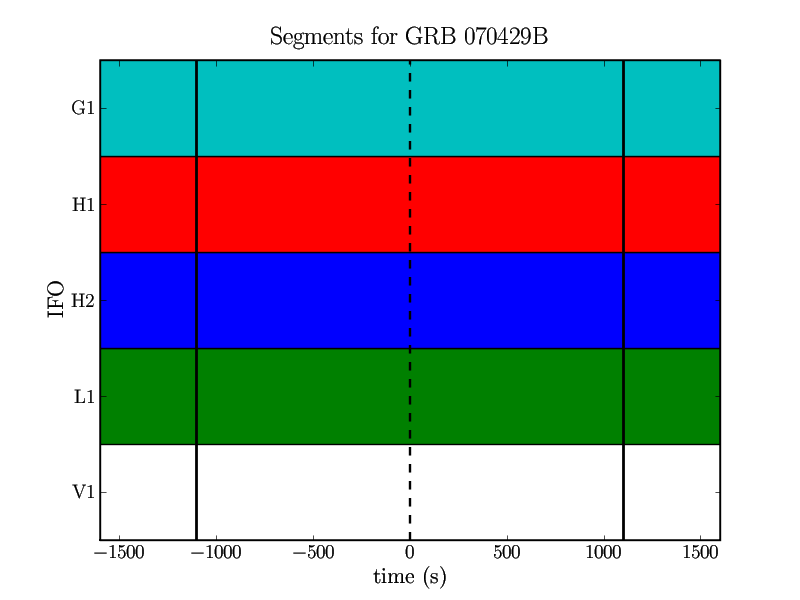
\includegraphics[scale=0.30]{Images/GRB070429B_segments.png}
\caption{Data segments availability for GRB070429B -- the "0" line represents the trigger time (the burst arrival time recorded by \emph{Swift} satellite); solid colors for the IFO (detectors) show continuous science--mode.}
\label{grbsegments}
\end{figure}

\subsection{Two--stage coincident pipeline}
\label{pipeline}
\paragraph{Pipeline overview}

Data streams from each detector participating in the search are first analyzed separately. As this is a coincidence search, the first stage of the pipeline is to determine if there is any loud \ac{SNR} event in any of the detectors. For each detector the process is to:
%
\begin{itemize}
 \item Generate a template bank to cover the full mass range.
 \item Filter the data against every template in the bank for each detector.
 \item Retain a ``trigger'' whenever a loud \ac{SNR}, above a certain threshold, is observed.
\end{itemize}
%
This results in a list of single detector triggers for each detector. The lists are then examined for any triggers that are coincident between detectors. A trigger is discarded if it is not seen in more than one detector. Coincidence is determined using the masses of the templates as well as the observed time.

In reality, the GW detector data is neither stationary nor Gaussian and to minimize these effects a two--stage coincident pipeline is used, with a schematic in Figures \ref{cbcstage1} and \ref{cbcstage2} for the analysis of GRB070429B that used data from H1 and L1 detectors. Each of the stages will be described in detail in the next subsections and here we provide just a brief overview: the first stage of the pipeline takes the calibrated $h(t)$ from H1 and L1 (calibration is not covered in this work but references can be found here in ~\cite{Abadie:2010px, Allen:1996, Adhikari:2003}) and constructs a template bank populated with theoretical waveforms through which the calibrated data will be matched--filtered. The resulting matched--filtering events will be tested for coincidence status in both H1 and L1, and if coincidences are found, these events will form the basis of the second stage of the pipeline. The coincident events will have their templates reconstructed collectively into a new template bank through which the resulting stage one triggers will be match--filtered. Signal--consistency veto tests will be applied at this level and the surviving triggers will be tested again for coincidence. The final steps of the second stage involve constructing a combined statistic of the coincident events (together with the results of the signal--consistency tests) and a final ranking of the events according to this statistic, leading to false alarm estimation and a detection statement.
%
\begin{figure}[htb!]
\centering
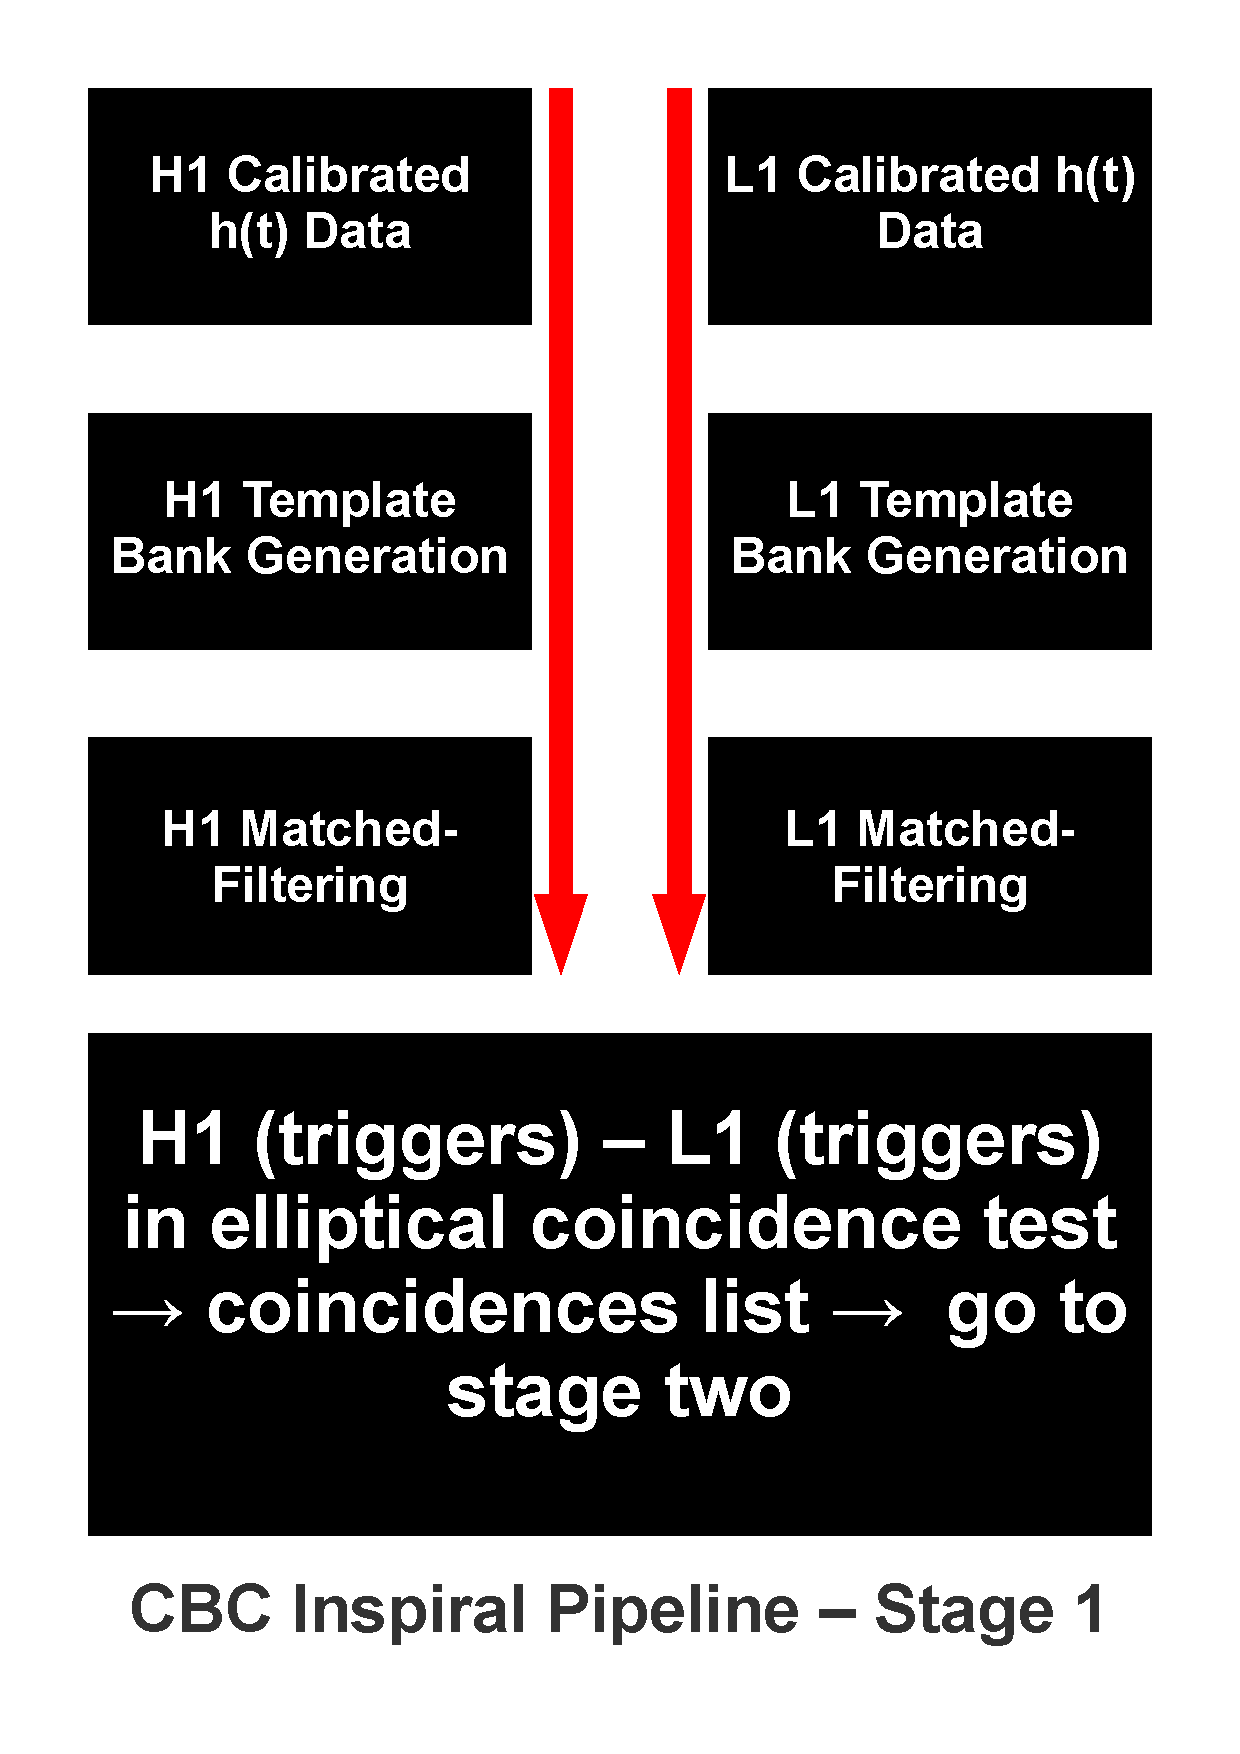
\includegraphics[scale=0.4]{Images/CBC_Stage_1.pdf}
\caption{Stage 1 of the CBC inspiral pipeline}
\label{cbcstage1}
\end{figure}
\begin{figure}[htb!]
\centering
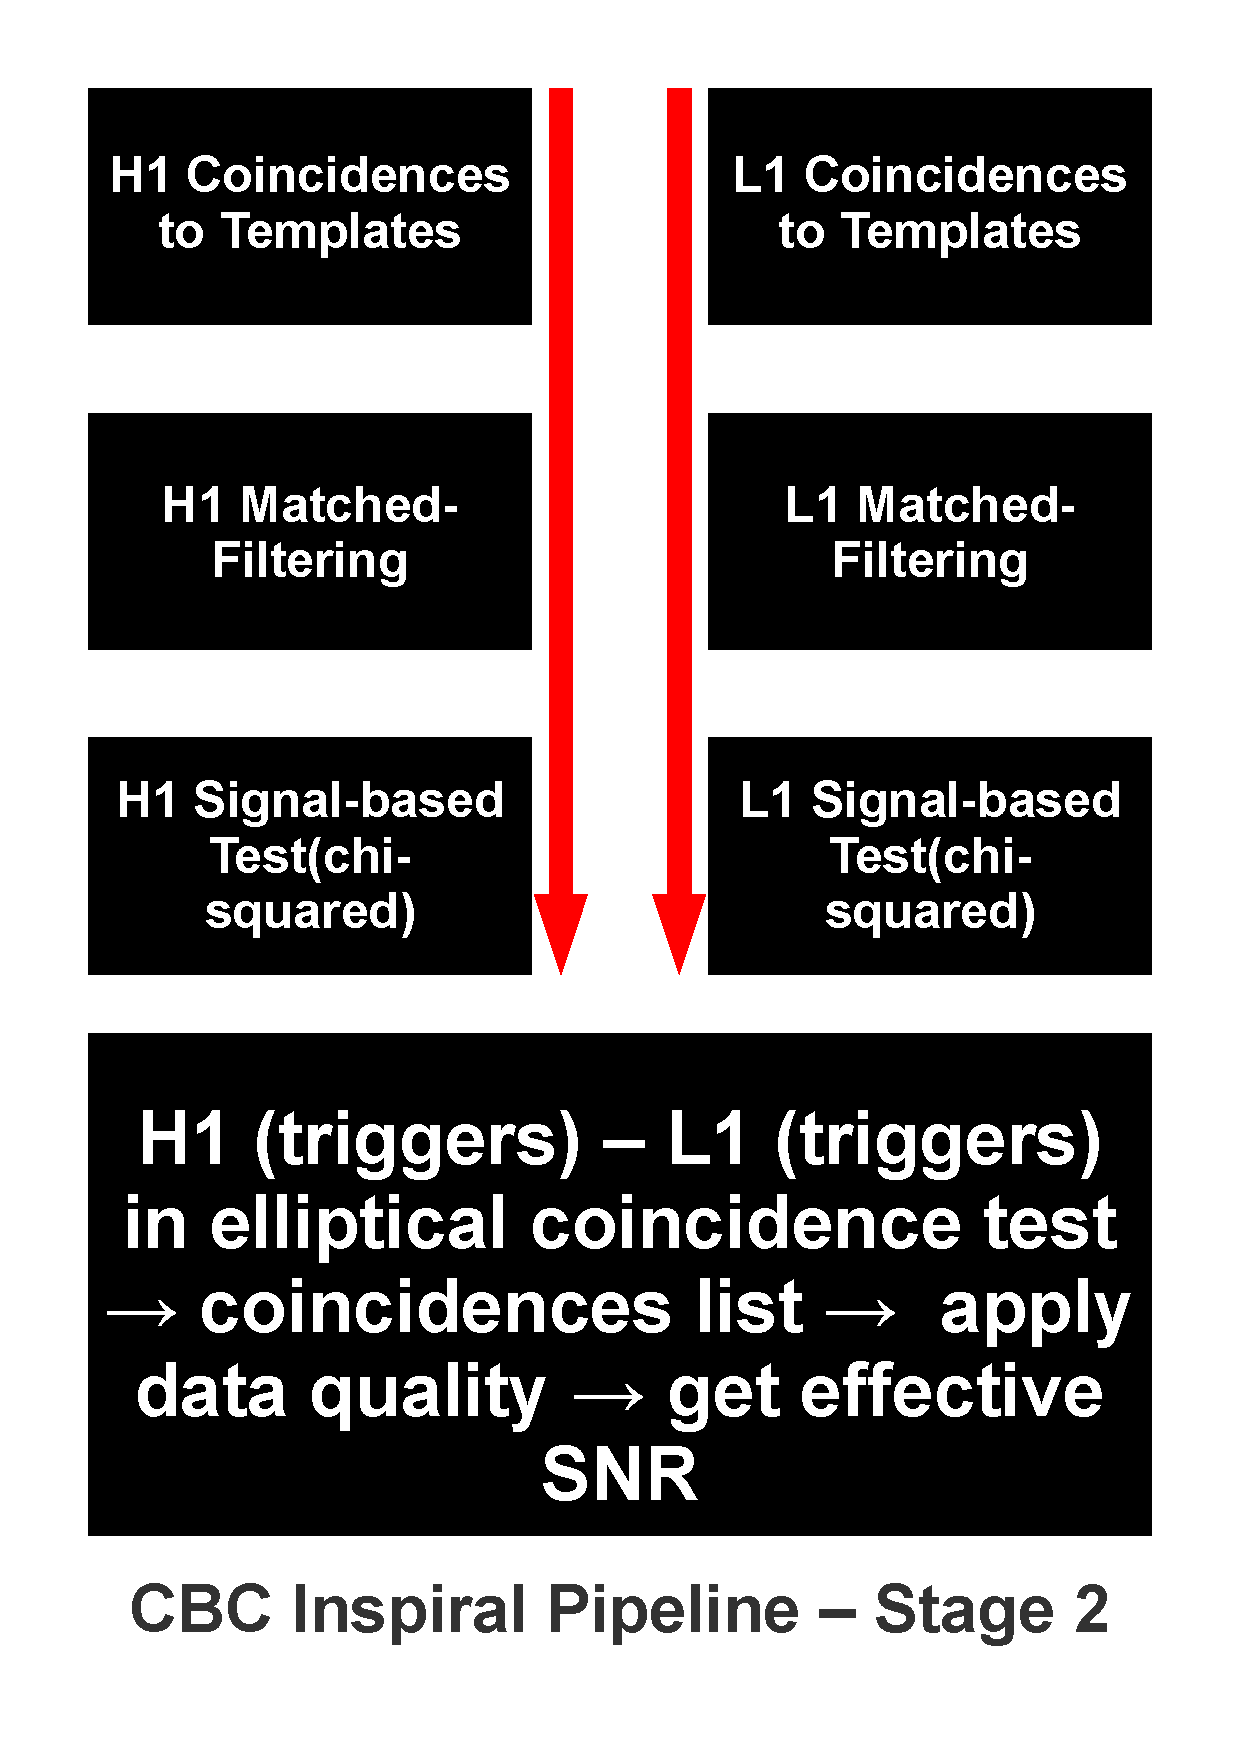
\includegraphics[scale=0.4]{Images/CBC_Stage_2.pdf}
\caption{Stage 2 of the CBC inspiral pipeline}
\label{cbcstage2}
\end{figure}
%

\subsection{Template bank}

In the case of GRB070429B, the matched--filtering was done using a non--spinning waveform template bank that was symmetric in component masses in the interval ~$2 \times M_{\odot} \leq M < 40 \times M_{\odot}$ in total mass $M$ \cite{Abadie:2010uf}. The number of template waveforms depends on the sensitivity of the detector and in this case, having to analyze data from H1 and L1, $\sim$~6000 templates have been used for H1 and $\sim$~9000 for L1 respectively, due to its flatter noise curve. For the GRB070429B search $\tilde{h}_0$ is calculated directly in the frequency domain using the ``TaylorF2'' Post--Newtonian approximate waveforms as described in \cite{Blanchet:2001dw} (see Chapter \ref{Chapter One} for a short explanation of Post--Newtonian formalism).

\subsection{Trigger generation}
Equation (\ref{eq:cbc_lowsnr}) gives the maximized SNR that can be calculated at all times in the segment being analyzed using equation (\ref{eq:cbc_fouriermagic}). The result of matched--filtering through the template bank is a discrete time--series of \emph{triggers} with various SNRs as measure of their ``loudness''. As an illustration, the time--series of triggers from H1 is plotted in Figure \ref{H1snr} for GRB070429B. It is easy to show that the expected distribution of $\rho^2$ in Gaussian noise will follow a $\chi^2$ distribution with two degrees of freedom. Triggers are retained only where the SNR at that point in time is larger than a threshold SNR $\rho_0$ and is the largest SNR within a small time interval. The number of triggers significantly increases below this threshold value of the SNR. The SNR threshold for the matched filtering step was chosen differently depending on which detectors are available for a given GW--GRB search. If data from H1 and L1 were analyzed, the threshold for each detector was set to $\rho_0 = 4.25$, reflecting their comparable sensitivity. If data from H1 and H2 were analyzed, the threshold of the latter detector, the less sensitive of the two, was set to 3.5 to gain maximum network sensitivity, while the threshold of the more sensitive detector, H1, was set to $\rho_0 = 5.5$ since any signal seen in H2 would be twice as loud in H1, with some uncertainty. For triggers with SNR $\rho > \rho_0$, the template masses and the time of the maximum SNR are recorded. For a given template, threshold crossings are clustered in time domain using a sliding window equal to the duration of the template \cite{Allen:2004gu}. For each trigger identified in this way, the coalescence phase and the effective distance -- the distance at which an optimally oriented and optimally located binary, with masses corresponding to those of the template, would give the observed SNR are also computed.

\begin{figure}[ht!]
\centering
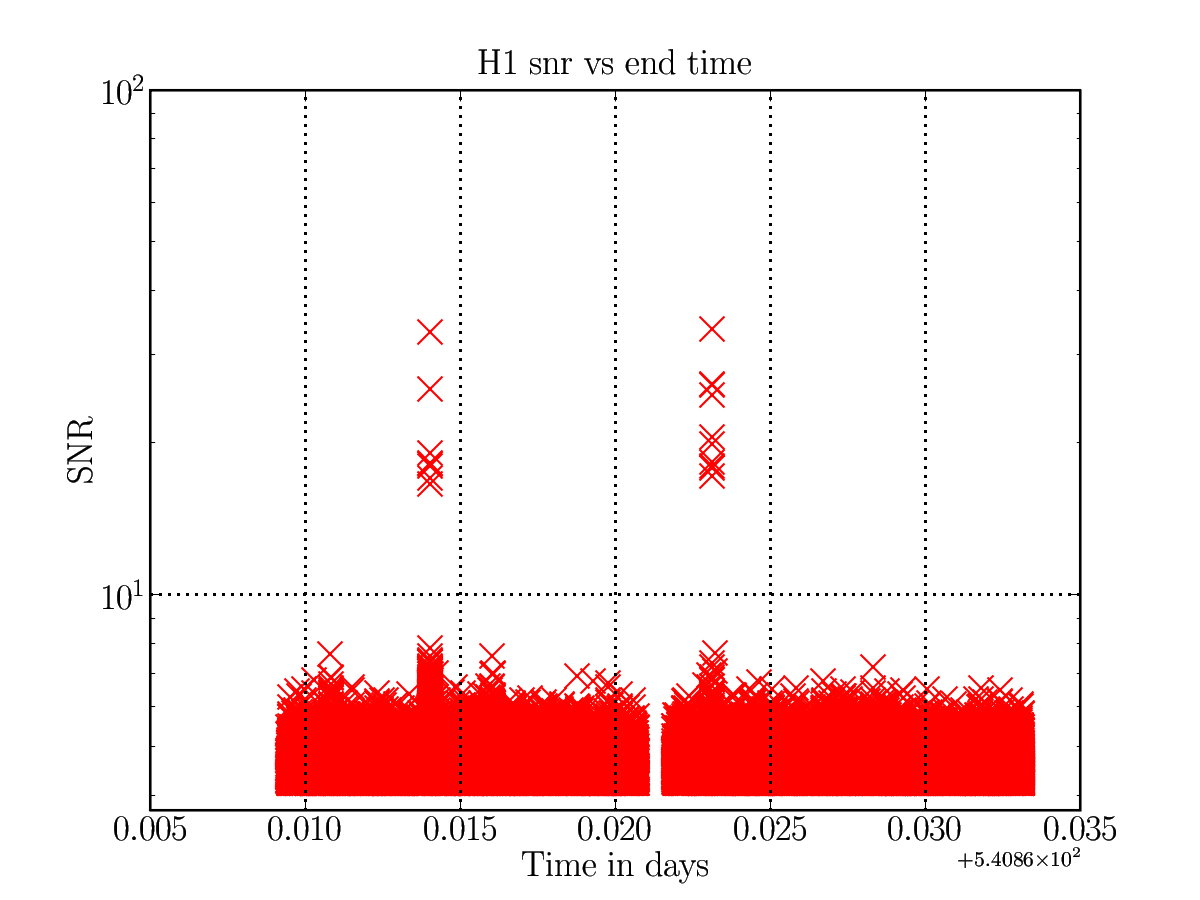
\includegraphics[scale=0.30]{Images/H1_SNR_time.png}
\caption{SNR time--series for Hanford H1 triggers for GRB070429B. We notice two loud glitches with SNR$\approx$40; the gap region corresponds to the ``on--source'' segment that we will examine visually only at the end of the analysis.}
\label{H1snr}
\end{figure}

Each non--Gaussian noise event has the tendency to match a series of different templates, usually high chirp mass ones, creating clusters of triggers. Usually these triggers tend to have high SNR values and in an SNR time--series given in Figure \ref{H1snr} show up as loud events much above the background at lower SNRs.

\subsection{Coincidence test and coincidence events}
\label{grb070429bcoincidence}
In GW coincidence analysis, data sets from each detector will be analyzed separately, following the steps outlined above, and the resulting output of the matched filtering stage will be single--detector triggers with different masses and coalescence times. Since the effect of a GW should be the same at all the operational detectors, the analysis requires that triggers from each detector be \emph{coincident} -- the next step of the pipeline is to perform coincidence tests between the triggers that are produced in each of the detectors. Triggers are considered coincident if they occurred at the same time and have similar masses. The definition of trigger ``coincidence'', as used in the actual analysis, is given in \cite{Robinson:2008un}: the presence of noise causes errors in the measurement of parameters of an inherent signal; due to this, it is very improbable that the same gravitational wave in different detectors can be associated with \emph{exactly} the same set of masses and times. However, it should be possible to detect signals in coincidence by demanding that the measured parameters lie in a sufficiently small parameter window, called \emph{coincidence window} \cite{Robinson:2008un}.

Considering a three--dimensional trigger parameter space with coordinates identical to the template bank coordinates $\vec{\theta} = (t_c, \tau_0(m_1,m_2), \tau_3(m_1,m_2))$, the parametric distance between two signals (expected broadening due to noise) will be given by:

\begin{equation}
\mathrm{d}l^2 = g_{12}(\vec{\theta})\mathrm{d} \theta_1\mathrm{d}\theta_2 \sim \frac{1}{\rho^2}
\end{equation}

\noindent where the metric $g_{12}(\vec{\theta})$ is the same template bank metric and is defined on the $\vec{\theta}$ vector space given by equation (\ref{ethincametric}). Since in the presented analysis we used data from two detectors with two different PSDs, and the metric depends on the PSD, there will be two different metrics to choose from. This is resolved by generating an ellipsoid in the $\vec{\theta} = (t_c, \tau_0(m_1,m_2), \tau_3(m_1,m_2))$ space around every trigger, observed in each of the operational detectors, using the appropriate metric given the noise PSD of the detector. The ellipsoid size can be tuned before the analysis, so that for any given threshold, all the points within the distance $\mathrm{d}l$ lie within the ellipsoid. Since only triggers with similar time of coalescence $t_c$ can be coincident, it is useful to first sort the triggers by $t_c$ and then check for coincidences; this greatly reduces the computational costs. For every pair of independent detector triggers, the overlap of their corresponding ellipsoids is measured; the triggers are considered coincident if the distance $\mathrm{d}l$ is smaller than a certain threshold (ellipsoid thinca or e-thinca parameter). The smaller the e-thinca parameter is, the closer the two triggers are in the $\vec{\theta}$ parameter space, hence the better a coincidence is confirmed. The threshold is empirically set at 0.8 by investigating the distribution for triggers associated with simulated signals; this value corresponds approximately to the limit where the majority of simulations are not recovered. The triggers that survive the coincidence test are stored and component masses, coalescence phases and effective distances are computed from the templates they were matched against.

The $\chi^2$ signal consistency test, which we describe in detail in Chapter \ref{Chapter Three}, tests whether a potential trigger has the expected power in a number of different frequency bins (16 bins, in the GW--GRB search). The $\chi^2$ test is a very effective method of separating non--stationary noise events from true GW signals; unfortunately is is also very computationally intensive: a matched--filter needs to be calculated for every frequency bin. Therefore, the test is performed only when necessary: single detector $\chi^2$ is computed for every coincident trigger only at the second stage of the pipeline. 


The SNR--cut, coincidence and signal--consistency tests provide strong veto capacity to remove accidental noise triggers in the detector data that can not be coincident GW signals. The first stage matched--filtering of the data produced roughly 158$\times 10^3$ triggers for H1 and 210$\times 10^3$ triggers for L1 in the case of GRB070429B. After the first stage of the pipeline, where a cut on threshold SNR and the Ethinca test were applied, the total number of triggers was reduced to roughly 82$\times 10^3$ for H1 and 110$\times 10^3$ for L1 respectively, this accounting for a reduction of $\sim$50$\%$ in the total number of triggers. Further on, after the second stage of the pipeline, where matched--filtering was repeated and both coincidence and the $\chi^2$ tests were applied, the remaining number of coincidences was left to 4593. 

\subsection{Ranking statistic}
The SNRs and  $\chi^2$ test results from each detector are combined into an effective SNR that weighs less those triggers with large values of $\chi^2$ that are not likely to be GW signals. For a signal with relatively small SNR and an average value of the $\chi^2$ veto, the value of effective SNR is equal to the SNR. However, for a noise trigger with a large $\chi^2$ value, the effective $\rho$ is reduced according to equation (\ref{eqn:roeff}):

\begin{equation}
\rho^2_{\mathrm{eff}} = \frac{\rho^2}{\sqrt {( \frac {\chi^2}{2p-2})(1+ \frac {\rho^2}{250})}}
\label{eqn:roeff}
\end{equation}

\noindent In equation (\ref{eqn:roeff}), $p$ is the number of degrees of freedom in the $\chi^2$ measure, 16 for the coincident search. The denominator 250 is chosen to best separate the background (off--source) from signal. The effective SNRs from the analysis detectors are added in quadrature to obtain a cumulative effective SNR \cite{Abbott:2009tt,Abadie:2010yb}, in the case of GRB070429B we have H1 and L1 participating:

\begin{equation}
\rho^2_{\mathrm{eff}} = \rho^2_{\mathrm{effective, H1}} + \rho^2_{\mathrm{effective, L1}}
\end{equation}

\subsection{Data quality vetoes}
To reduce the number of triggers present due to non--Gaussian and non--stationary noise, it is useful
to try to identify times during which noise transients are likely to occur. These glitches are usually produced because of environmental causes to the detectors; these influence the detectors' optimal operation, e.g., increased seismic activity that produces low--frequency vibrations or electromagnetic disturbances that may produce glitches in high--frequency bands. For these reasons the detectors are continually monitored by a series of sensors, which survey the internal and external conditions. Work is constantly done on both monitoring the existent channels thought to produce noise glitches and trying to identify new noise channels. This effort is called \emph{detector characterization}. This information is used to flag the excessive noise periods and to discard the data that is associated with these times, process called \emph{vetoing}. For more details of these activities see \cite{Blackburn:2008ah,Macleod:2011up}.

To consider this from the point of view of the data analyst, it is sufficient to know whether
the data should be analyzed or not. The end product of the detector characterization process
is to assign all data a data quality category. Analyses for CBC signals treat these
data quality categories in the following way\footnote{
Note that there is also a category 4, but for CBC searches this category is only used when following up interesting triggers. Category 4 was not used on GRB070429B data.}
%
\begin{itemize}
 \item Category 1 veto: Data marked as category 1 indicates that the GW detectors don't operate in a correct way. This data is not used for any analysis and is not used to compute the noise PSD; it is discarded. As an example would be when the calibration cannot be attained and the strain $h(t)$ is not available; 
 \item Category 2 veto: Data marked as category 2 indicates that the detectors were operating normally but a mechanism \emph{known} to induce glitches in the data was active. This type of data \emph{may} be used to compute the noise PSD, however any trigger occurring during this time will be discarded.
 \item Category 3: Data marked as category 3 indicates that \emph{some} mechanism known to have some correlation with noise transients was active at the time this data was taken. Category 3 data \textit{is} analyzed and false alarm rates are calculated for coincident triggers occurring during category 3 data. Category 3 data is, however, discarded when calculating upper limits. An example
of a category 3 flag might be that there is elevated seismic noise at the time the data is
taken.
\end{itemize}

\subsection{Background estimation}

In order to make a GW detection statement, in the triggered GRB searches, we need to make a statement about the events that are obtained purely from detector noise, the \emph{background} where we don't expect any GW signals. Unlike the un--triggered searches that use non--physical times for background segments obtained from time--shifting data stretches, the triggered GRB searches use as background segments on either side of the on--source (a timesliding method has now been implemented in the triggered search as well, see Chapter \ref{Chapter Five}). Since the length of these segments is usually of $\approx1000$~s the detectors' PSD is not expected to change drastically over such short time and hence the background data should have roughly the same statistical properties as the on--source. We would want to characterize the background (``off--source'') segments in terms of the coincident events we would expect from analyzing it, also in terms of the actual ``off--source'' triggers we find. If the detectors' noise were to be stationary and Gaussian, the background could be characterized analytically using the distribution for SNRs above the threshold. In reality, the background of a GRB search is abundant in non--stationary phenomena (noise glitches) and the analysis will not assume stationarity or Gaussianity.

The rate of background events at a fixed effective SNR is not constant across the template space. In general, the non--Gaussian background is better suppressed for low(er) mass templates (longer duration templates) since the signal--based vetoes are more powerful for these kind of templates rather than for the shorter ones. To account for this, the set of coincident events are split up and the significance of triggers is calculated relative to a background of comparable events. The surviving coincidences are gathered in a candidate list which will be partitioned in three chirp mass bins, according to their recovered chirp mass \footnote{The reason for chirp mass binning is that due to the large variation in the length of the templates used during the search (shortest template is $\sim$0.3s and longest is $\sim$45s), there is a larger variation in the templatesÕ responses to noise glitches in the detectors where glitches tend to match higher mass templates (and shorter), the result being triggers with larger values of SNR. When binning, after applying signal--based cuts, we end up with a high chirp mass bin containing much fewer triggers than the other two bins, since a lot of these triggers are glitches that get rejected by applying the cuts. The chirp mass binning will subsequently be revised and cancelled for the IPN GRB search, see Chapter \ref{Chapter Seven}.} ($\mathcal{M} \in [0.86,3.48)$, $[3.48,7.40)$, $[7.40,17.5)$) and in a certain number (324 for GRB070429B) of 6--second off--source trials \footnote{Because glitches tend to match many templates over a much larger template sub--space than true GW signals, clustering on trials is important on one hand to eliminate any possible correlations between the loudest events that might originate from the same glitch over time periods much shorter than the 6s trial length. On the other hand, it is important to provide multiple similar data stretches that replicate the on--source both in duration and trigger distribution.}. In each of the off--source trials, in each chirp mass bin, the coincidence with the highest effective SNR is retained only, the other coincidences are discarded. This process is called clustering on trials and chirp mass bins. 

Once clustered, we can express a basic formulation for the \emph{false alarm probability}, the measured occurrence of coincidences as loud or louder than a reference coincidence:

\begin{equation}
\mathrm{FAP} = \frac{N(\rho \geq \rho_c)}{N_0}
\end{equation}

\noindent where $N(\rho \geq \rho_c)$ is the total number of coincidences drawn from the background distribution with $\rho$ greater or equal to $\rho_c$ and $N_0$ the effective number of off--source trials. The cumulative number of candidates versus effective SNR squared for the low chirp mass bin of GRB070429B is shown in Figure \ref{FARlowbin}. This figure describes the population of background triggers ranked by effective SNR: on the $y$--axis, the number of loudest events louder than the $x$--value of the effective SNR squared (divided by the effective number of trials) is the false alarm probability (FAP). The FAP is constant and equal to 0.8 up to roughly an effective SNR squared of 40 corresponding to an individual detector SNR of $\approx4.5 - 5$, that is, triggers close to threshold. It then decreases linearly down to a value of one trigger per the total number of trials ($\approx$1/300) for a single trigger with a statistic squared of 70, corresponding to a single detector SNR of $\approx6 - 6.5$. This is the loudest background trigger and any on--source candidate, in order to represent a possible GW detection, should be as loud or louder. We used the term effective number of trials due to the fact that 6 s trials that overlap a time of CAT2 veto will be discarded, resulting in a decrease in number of trials.

\begin{figure}[ht!]
\centering
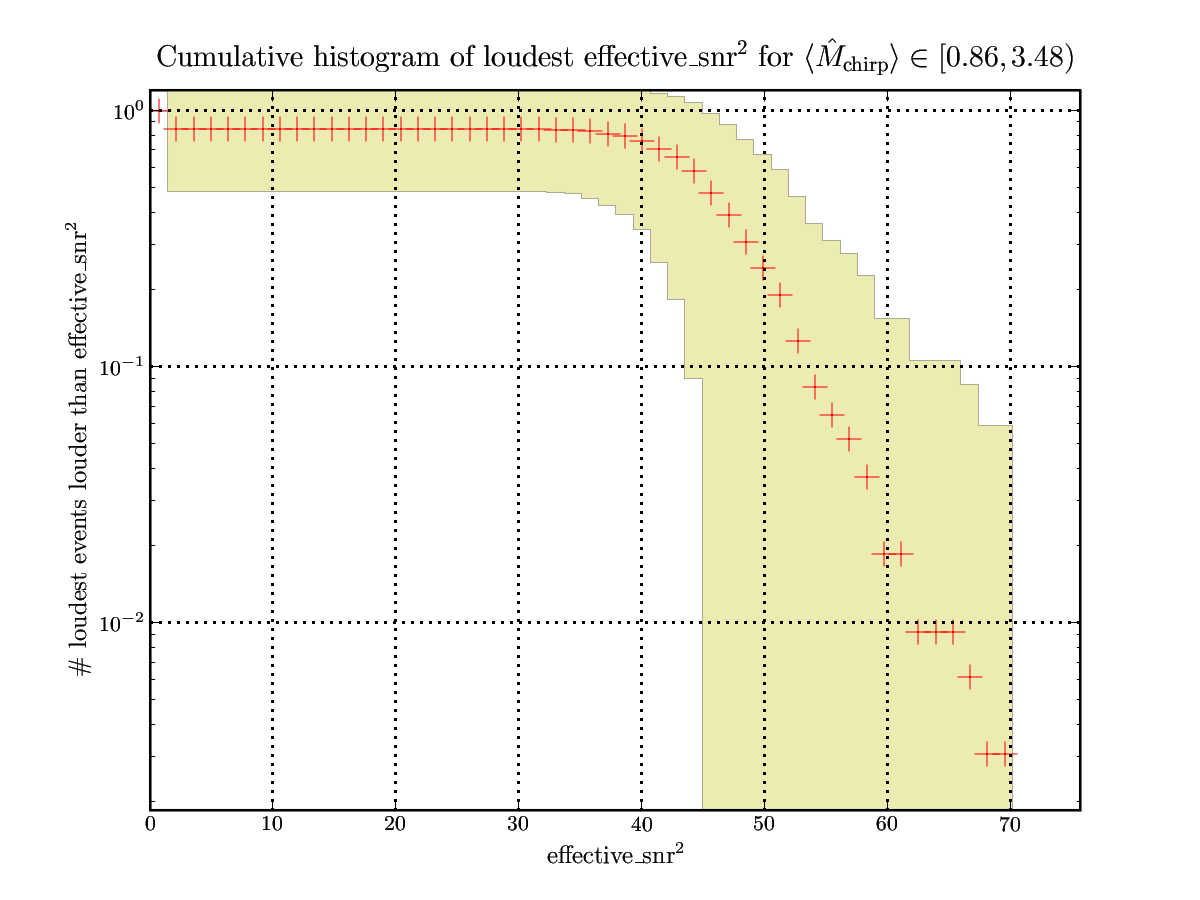
\includegraphics[scale=0.35]{Images/Triggers_Mc1.png}
\caption{Cumulative histogram of the loudest coincident triggers in low chirp mass bin versus combined effective SNR squared (proportion of triggers that have a combined effective squared SNR greater than or equal to a given value on the $x$--axis for the low chirp-mass bin). This represents the variation of the false alarm probability (FAP) with the ranking statistic. The FAP is constant and equal to 1 up to roughly an effective SNR squared of 40 corresponding to an individual detector SNR of $\approx4.5 - 5$, that is, triggers close to threshold. It then decreases linearly down to a value of one trigger per the total number of trials ($\approx$1/300) for a single trigger with a statistic of 70, corresponding to a single detector SNR of $\rho \approx 6 - 6.5$. This is the loudest background trigger and any on--source candidate, in order to represent a possible GW detection, should be as loud or louder}
\label{FARlowbin}
\end{figure}

The minimum non--zero false alarm rate one can get for an on--source candidate, louder than all the off--source loudest coincidences, bar one, is 1/(maximum number of trials = 324)$\approx3.1 \times 10^{-3}$ and, as will be seen in Chapter \ref{Chapter Five}, this is not enough for a detection statement. A more detailed explanation of the background estimation is given in Chapter \ref{Chapter Five}.

\subsection{Simulated signals}
\label{siminj}

There are two ways to test the pipeline's efficiency of detecting GW signals: by performing a large number of \emph{software injections} and by performing a much smaller number of \emph{hardware injections}. Software simulations are performed by adding a simulated waveform to the data after it has been read into the pipeline’s analysis codes; they cover a wide range of masses and coalescence times. Hardware simulations are performed by actually moving the detector mirrors (process called actuation) to mimic the effect of a possible GW signal. Hardware injections replicate more accurately a true GW signal, but are limited in choosing the injected parameters and only a limited number of these injections can be performed; data containing a hardware injection cannot be used when searching for real GW signals. Software injections are used in calculating the detection efficiency and the final upper limits. 

The search efficiency is defined as the fraction of simulated signals which are successfully detected by the pipeline. A software injection is considered found if there is a trigger found within 100 ms of the time of the simulation. This can lead to an injection being falsely found especially in the case when trigger rates are high; however, we are typically interested in evaluating the sensitivity of the search at or around the combined effective SNR of the most significant event -- in this case, the number of spuriously identified signals is essentially null. It is important, for tuning the analysis, to examine the simulations that \emph{should} have been found (given their amplitudes) but were not; since the amplitude is inversely proportional to the distance. simulations performed at low distances are still missed by the pipeline and one needs to find out the reasons why. Reasons for not finding an injection range from the existence of a very loud detector glitch at the time (or very nearby) of the injection, a very poor choice of parameters in the simulation (is mostly referred to high--spin simulations, in the case where we inject spinning waveforms, not applicable in our case). The missed/found injections plot for injections in H1 is shown in Figures \ref{injectionsH1} and \ref{injectionstimeH1}.

\begin{figure}[ht!]
\centering
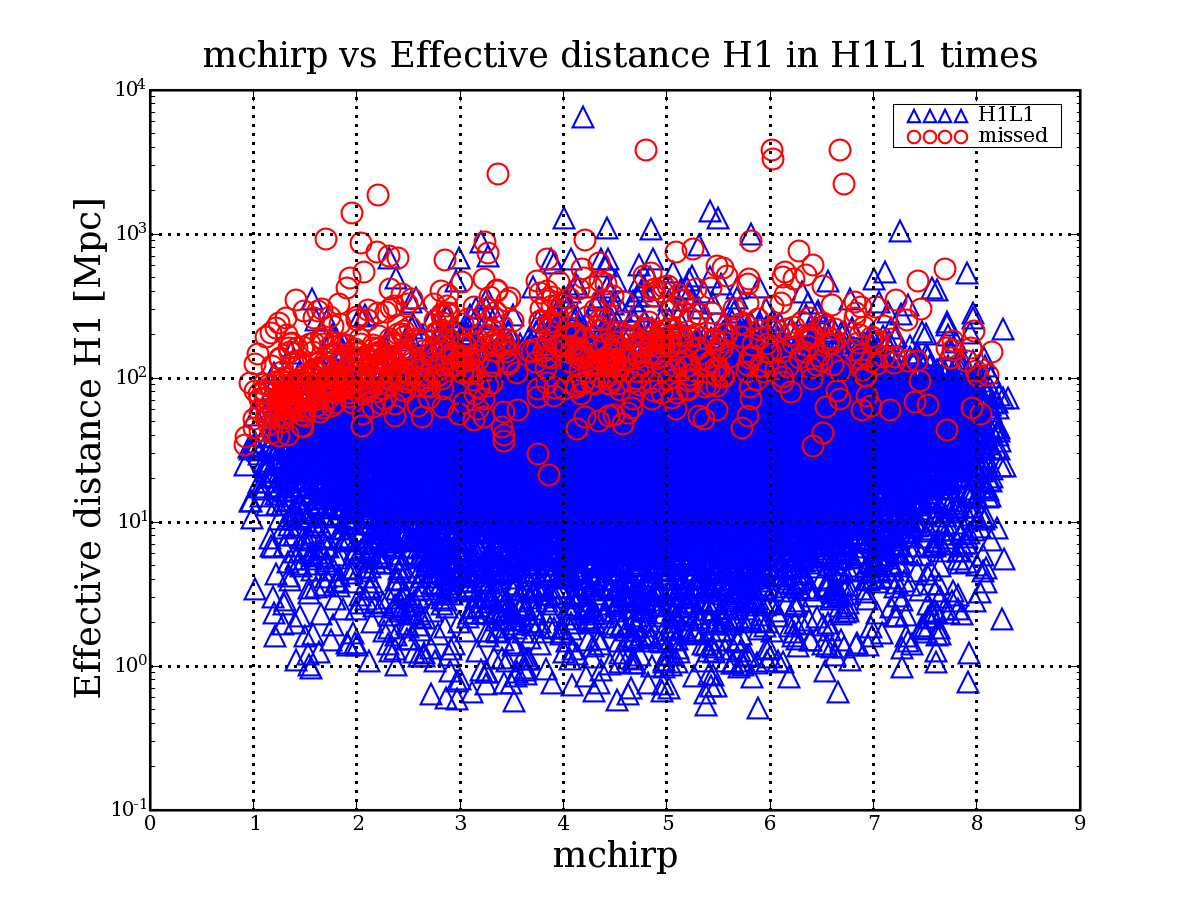
\includegraphics[scale=0.35]{Images/Foundmissed_INJ_H1.png}
\caption{Found/missed injections in H1: effective distance in Hanford H1 vs. chirp mass of found/missed simulations (blue triangles: found, red circles: missed). Injections with higher chirp mass tend to be found better since they have shorter templates that produce higher SNR triggers; the effective distance of a reference 1.4 -- 1.4 $\mathrm{M}_{\odot}$ binary at which we start missing injections is $\approx$40 Mpc, roughly the inspiral horizon distance in H1 (LIGO's H1 and L1 inspiral horizon distances at the time of GRB070429B were $\sim$35 Mpc for H1 and $\sim$34 Mpc for L1 respectively).}
\label{injectionsH1}
\end{figure}

\begin{figure}[ht!]
\centering
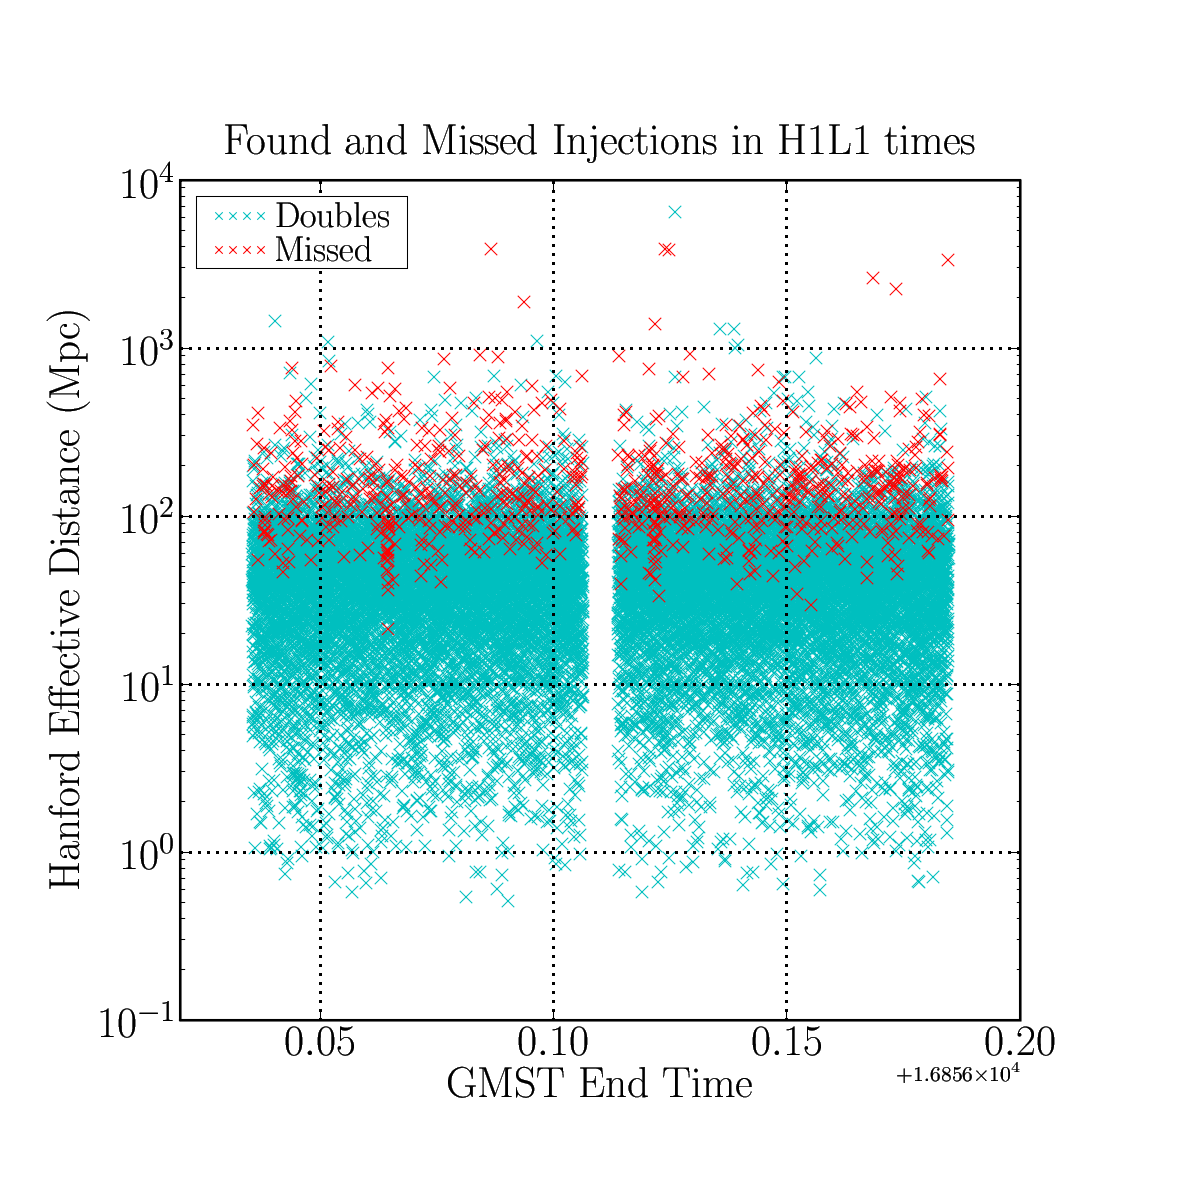
\includegraphics[scale=0.35]{Images/070429B_missed_time.png}
\caption{Found/missed injections in H1: effective distance in Hanford H1 vs. time. There are two times of poor data quality (``glitchy'' times) where injections are missed consistently at distances below the inspiral horizon distance, at 20--30 Mpc; we expect the fraction of missed/found injections to increase significantly at distances above 50 Mpc.}
\label{injectionstimeH1}
\end{figure}

It is important to cover the full search parameter space when performing simulations, both to test the analysis in order to find the cases where it doesn't perform as expected, and to accurately evaluate the sensitivity of the search. The simulations' parameter space is chosen depending on a set of astrophysical priors specific to the particular search we are performing. In the triggered search around short GRB times, we use the assumption that the progenitor source is a compact binary coalescence (either NS--NS or NS--BH binaries, see Chapter \ref{Chapter Two} for motivation) hence in terms of masses, we drew the NS mass uniformly from [1, 3) $\mathrm{M}_{\odot}$ and the BH mass uniformly from [1, 25) $\mathrm{M}_{\odot}$. We also restrict the parameter space by simulating signals only at the given sky location of the GRB (keeping dec constant and RA adjusted based on coalescence time $t_0$ to keep each simulation at the same location relative to the GW detector). In terms of inclination angle $\iota$ with respect to our line of sight, the simulations' $\iota$ was drawn uniformly in $\cos \iota$. The polarization angle was drawn uniformly in $[0,2\pi)$ and the coalescence time was uniform within the off--source time.

\subsection{Results: detection statement}
A simple ``poor man'' likelihood function is constructed to express how likely it is for an on--source candidate to be a signal (or not) -- we will derive a more precise expression of a detection likelihood in Chapter 5, using Bayesian inference; the likelihood is proportional to the pipeline efficiency in recovering simulated signals and inversely proportional with the background events false alarm probability:

\begin{equation}
\mathcal{L} := \frac{N_{\mathrm{found}}/N_{\mathrm{total}}}{N(\rho>\rho_0)/N_0}
\label{coinklike}
\end{equation}
%
where $N_{\mathrm{found}}/N_{\mathrm{total}}$ is the number of found injections divided by the total number of injections, or the injection recovery efficiency and $N(\rho>\rho_0)/N_0$ is the number of background events with an effective SNR $\rho$ larger than the onsource $\rho_0$, divided by the effective number of off--source trials, or the background FAP. The efficiency is a function of two signal parameters (distance and companion mass) and is marginalized over all other parameters; it is obtained by simply counting across injection trials. The FAP is obtained by counting across off-source trials. The FAP for every on--source candidate, for GRB070429B, is shown in Figure \ref{fig:far} and the low mass bin candidate, with an effective SNR=7.5 is the ``loudest'' on--source candidate but with a relatively high FAP=0.12, meaning it was only the $\approx$37th loudest candidate from on-- and off--source times collectively. The high chirp mass bin candidate, with FAP=0.117, is the most ``significant'' in terms of FAP, but only $\approx$35th loudest event of on-- and off--source collectively.

\begin{figure}[ht!]
\centering
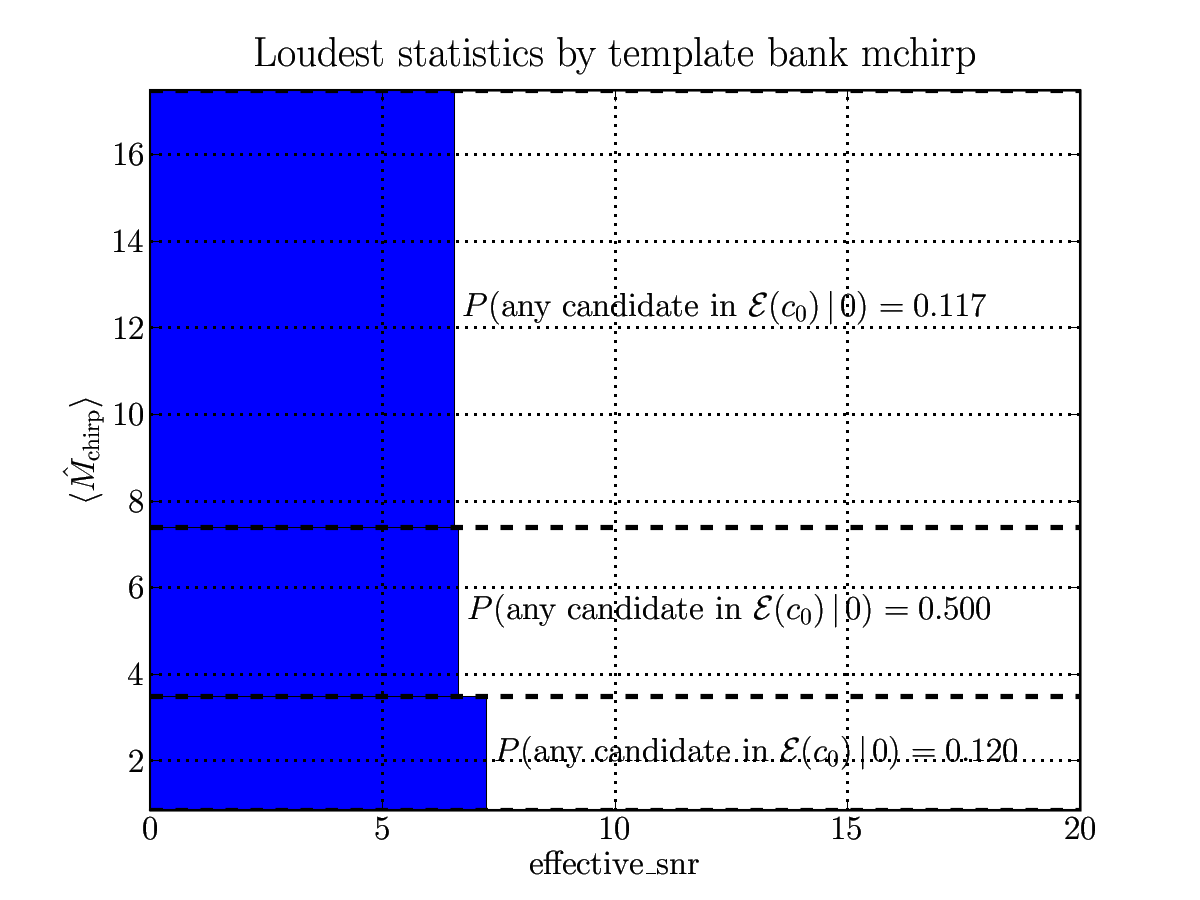
\includegraphics[scale=0.35]{Images/FAR.png}
\caption{False alarm probability for the on--source events in each chirp mass bin of GRB070429B, computed simply by counting the louder events in the background and dividing by the number of effective trials. The high chirp mass bin candidate, with FAP=0.117, is the most ``significant'' but only $\approx$35th loudest event of on-- and off--source collectively. The values on the $x$--axis correspond to the SNR of the loudest event in each of the chirp mass bins, plotted as solid bars on the $y$--axis.}
\label{fig:far}
\end{figure}

Figure \ref{onoffevents} shows the significance of the on--source loudest event relative to the distribution of background (off--source) events. The figure can be easily interpreted since the $x$--axis represents a statistic constructed from the likelihood given by equation \ref{coinklike}, that combines across the three chirp mass bins, and the $y$--axis is the event's probability of being drawn from the background sample -- this way we can see that the on--source event falls well in the background distribution and is not near the high--SNR ``tail'' of the rarest background events. In fact, to be able to claim a GW detection, the on--source event should be clear of the the background ``tail'', with false alarm probabilities of $\sim 10^{-6}$, as we will see in Chapter \ref{Chapter Five}, where we give an estimate for a FAP that should be associated with a GW--GRB detection.

\begin{figure}[ht!]
\centering
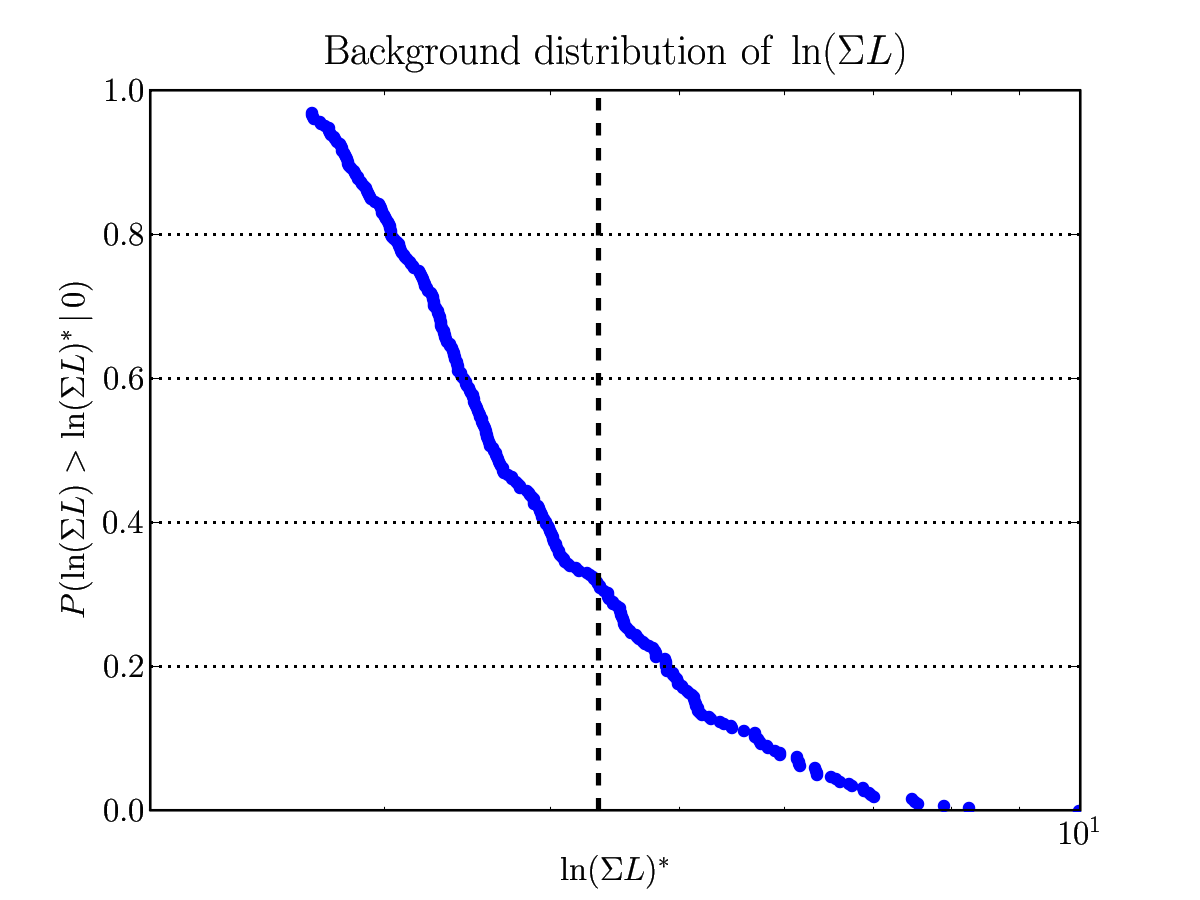
\includegraphics[scale=0.35]{Images/background.png}
\caption{The loudest on--source event (vertical dashed line) with respect to the background distribution of events (blue/dotted line). The figure can be easily interpreted since the $x$--axis represents a statistic constructed from the likelihood given by equation \ref{coinklike}, that combines across the three chirp mass bins, and the $y$--axis is the event's probability of being drawn from the background sample -- this way we can see that the on--source event falls well in the background distribution and is not near the high--SNR ``tail'' of the rarest background events..}
\label{onoffevents}
\end{figure}

\subsection{Results: distance exclusion}

Given the results from on--source, no detection of a GW signal was made. In this situation, we wish to place upper limits on the distance to the progenitor, based on the assumed astrophysical prior for the source: either a NS--NS or a NS--BH merger and the sensitivity of the search. We use the large number of simulations we performed and assume the GRB was caused by a compact binary coalescence with a neutron star (with a mass in the range [1, 3) $\mathrm{M}_{\odot}$) and a companion of mass $m_{comp}$. The $m_{comp}$ space is binned and we report a 90\% exclusion distance for a NS with mass in the range [1, 4) $\mathrm{M}_{\odot}$ and for BH with mass in the range [7, 10) $\mathrm{M}_{\odot}$. The actual computation of the exclusion distance will be omitted in this work but can be found in \cite{Abadie:2010uf}. We exclude a NS--NS merger to a distance of 9 Mpc and a NS--BH merger to 15 Mpc. These distances were derived assuming no beaming of the gamma radiation. The 90\% exclusion distance is larger for NS--BH systems than for NS--NS since more GW energy is radiated from a higher mass system; it also depends on the detectors' sensitivity (implicitly on the sky location of the GRB, see Chapter \ref{Chapter One}) and PSD at the time of the search, the likelihood of the on--source candidate(s) (if any) and on the parameter choice for simulations.


\subsection{Search summary}
We have analyzed 2190 s of GW data around the \emph{Swift} trigger time of the short hard GRB070429B. The two most sensitive operational GW detectors used for the search were H1 and L1. We have used the coincident triggered pipeline that looked for CBC signals using matched--filtering the data through a bank of theoretical waveforms. We have used two segments (one on either side of the GRB trigger) to estimate the background FAP and performed software simulations to obtain the search efficiency. We used a simple likelihood function (efficiency/FAP) to rank both on-- and off--source candidates. No gravitational wave signal has been detected in association with GRB070429B. The on--source data contains three triggers in each of the chirp mass bins but each of these triggers is not louder than the loudest background event; the most significant on--source trigger, in the high chirp mass bin, with an SNR of $\rho\approx$6.5 and a false alarm probability of FAP=0.12, was only order 30 loudest candidate from on-- and off--source times collectively. Given the GRB's association with a host galaxy at a luminosity distance of $\approx$4 Gpc, we would have not expected a GW detection. Based on the two astrophysical models for a CBC event (either NS--NS or NS--BH merger) we placed lower limits for distance to an NS--NS merger at 9 Mpc and for a NS--BH merger at 15 Mpc.

\section{Coherent triggered search}

\subsection{Introduction}

In Chapter \ref{Chapter Three} we have outlined the theoretical framework of a coherent analysis. In turn, in this section, we describe a triggered coherent search for \ac{CBC} signals associated with short GRBs and we will provide an example for illustration purposes. The particular search method, that we only summarize here, was used to analyze data during S6/VSR2 and 3 and is described in detail in \cite{Harry:2011qh} with search results in a final paper in the publication process \cite{lvc:s6grb}. This search was used to analyze \ac{GW} data around short gamma-ray burst triggers provided by both \emph{Swift} and Fermi/GBM satellites. Given the localization capabilities of the two GRB--observing missions, outlined in Chapter \ref{Chapter Two}, the search has been done on single sky points for the \emph{Swift}--observed GRBs (localization of arcsecond precision) and on multiple sky points within the Fermi--GBM error boxes (localization of a few square degrees precision). We will present here just a brief summary of this analysis method and of the results on GRB090831A, a GRB observed by the Fermi--GBM satellite. We invite the reader to consult the aforementioned references for an in--depth description of the coherent method and of the GRB analysis results for S6/VSR2 and 3. 

More recently, the same analysis method was used to analyze GW data associated with the IPN--detected short burst triggers collected during S5/VSR1. We will present in detail the search for GW associated with the S5/VSR1 IPN GRBs in Chapters \ref{Chapter Six} and \ref{Chapter Seven}.

The coherent analysis can be applied not only for single--point sky locations but also for extended sky regions, populated with multiple search points. A number of \ac{GRB}s that have been analyzed or to be analyzed, particularly those observed by Fermi--GBM and the InterPlanetary Network (see Chapters \ref{Chapter Two}, \ref{Chapter Six} and \ref{Chapter Seven}) are not localized with sufficient accuracy that the search could be done only at a single point on the sky.  Thus, the analysis has been extended to cover a region of the sky.  This requires looping over the relevant sky points, incorporating the correct detector sensitivities $F_{+,\times}$ and time delays between \ac{GW} detectors.  Since the majority of the analysis time is taken in performing the single detector filters and since these do \textit{not} need to be re--calculated for each sky point, the analysis does not take too much longer than the single--point one.  

Given the non--Gaussianity of the GW detector data and the lack of power of the matched--filtering to distinguish ``glitches'' from true signals, it is very important, on one hand, to understand the cause of these glitches \cite{Blackburn:2008ah} and to remove times of poor data quality. On the other hand, while the glitch--removal efforts greatly reduce the number of non--Gaussian events, they can not remove them entirely. Therefore the analysis must also employ methods to distinguish signal from noise transients. In previous \ac{CBC} searches, signal consistency tests e.g., \cite{Allen:2004gu, Hanna:2008} have proven very effective at removing the non--Gaussian background. We provided an overview of the formalism for the $\chi^{2}$ consistency test applied to coincident searches in Chapter \ref{Chapter Three} and in the previous section, and we will extend this test for the coherent analysis. This, together with describing new coherent--specific consistency tests such as the null stream and other multi--detector signal--based tests.

\subsection{Coherent search associated with GRB090831A}
\label{coh_search_grb}

\begin{figure}[ht!]
\centering
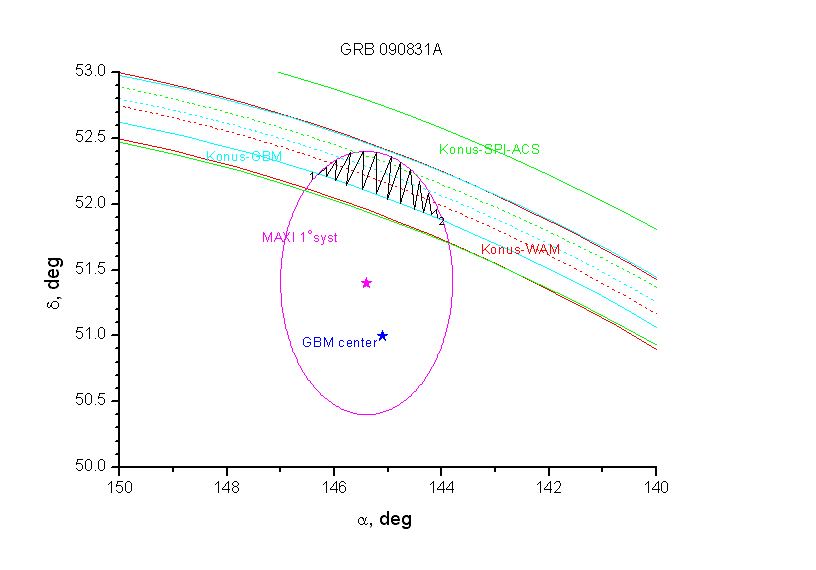
\includegraphics[scale=0.55]{Images/GRB090831A_IPN.png}
\caption{GRB090831A error region: blue star represents the Fermi--GBM localization error box best fit position; pink circle and star represent the MAXI (ISS) localization error box and best fit position, respectively; the hashed region represents the refined position with the help of IPN localization. The position accepted for the GW--GRB search was a conservative Fermi--GBM--only, centered at RA=145.1 and dec=51.0 degrees, with an error circle radius of $\approx$12.8 degrees -- figure from \cite{gcn9864}.}
\label{GRB090831A_IPN}
\end{figure}

\begin{table}[ht!]
 \begin{tabular}{|l|l|l|l|l|l|}
 \hline
 \hline
 GPS & Date & redshift & $T_{90}$ (s) & RA ($\deg$) & dec($\deg$) \\
 \hline
 935739411 & Aug. 31 2009, 07:36:36 UTC & n/a & 69 & 145.1 & 51.0 \\
 \hline
 \hline
 \end{tabular}
 \caption{Astronomical and detector data for GRB090831A. This was initially considered a long GRB/later considered short with an extended $T_{90}$ duration of $\approx$ 69 s and was observed by Fermi--GBM (and other missions, see text) to an approximate circular 1--$\sigma$ and systematics error box with a radius of 12.774 degrees. The active GW detectors were Hanford H1 and Virgo V1. Antenna factors are 0.146 and 0.881, respectively.}
 \label{Table_grb090831a}
\end{table}

\begin{figure}[ht!]
\centering
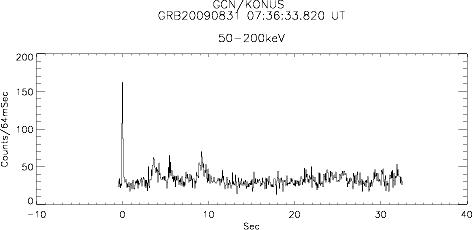
\includegraphics[scale=0.80]{Images/090831a_lc.png}
\caption{Konus--WIND GCN GRB090831A light curve (LC, $\gamma$ photon counts/s vs. time in the 50--200 keV band) showing a single intense peak followed by secondary and tertiary peaks. The $T_{90} \approx$69 s but this burst was still considered short based on visual inspection of this light curve \cite{konus}.}
\label{090831a_lc}
\end{figure}

\paragraph{GRB090831A overview}
GRB090831A is a \emph{long} gamma-ray burst detected initially by Fermi--GBM satellite and then by a series of other GRB missions. Based on subsequent visual inspection of the light curve, shown in Figure \ref{090831a_lc}, it was later considered \emph{short}, so a search for CBC events in association with it was ultimately performed. The light curve is showing a bright single peak followed by secondary and tertiary peaks. The Fermi--GBM light curve consists of two structured main pulses with a $T_{90}$ duration of about 69.1 s. According to GCN 9864 \cite{gcn9864}, GRB090831A was reported as both a Fermi--GBM and as a MAXI (Monitor of All-sky X--ray Image, an X--ray detector onboard the International Space Station, ISS) event. It was also reported as a Konus--WIND event, and detected by both Suzaku and INTEGRAL, both spacecraft part of the InterPlanetary Network (IPN, for further details on the the IPN and its missions, please consult Chapter \ref{Chapter Two} and Chapter \ref{Chapter Six}). Due to the involvement of the IPN in detection, the initial Fermi--GBM positional error region could be refined to a much smaller error box, see Figure ~\ref{GRB090831A_IPN} showing the Fermi--GBM best-fit position (blue star), the MAXI localization circle and best--fit position (pink star) together with the IPN (Konus--WIND, Suzaku, INTEGRAL) annuli (solid lines with centers dot--dashed). The hashed area shows the intersection of the Konus annulus with the 1--degree MAXI localization circle. The area of this region is 0.160 square degrees \cite{gcn9864}. Due to the fact that all Fermi--GBM--observed GRB locations are considered only based on the Fermi error circles, the position for the GW--GRB search was a conservative Fermi--GBM--only, centered at RA=145.1 and dec=51.0 degrees, with an error circle radius of $\approx$12.8 degrees (including systematic errors); we note that the IPN localization was available with a considerable delay, only after we have begun the GW search.

\begin{figure}[ht]
\centering
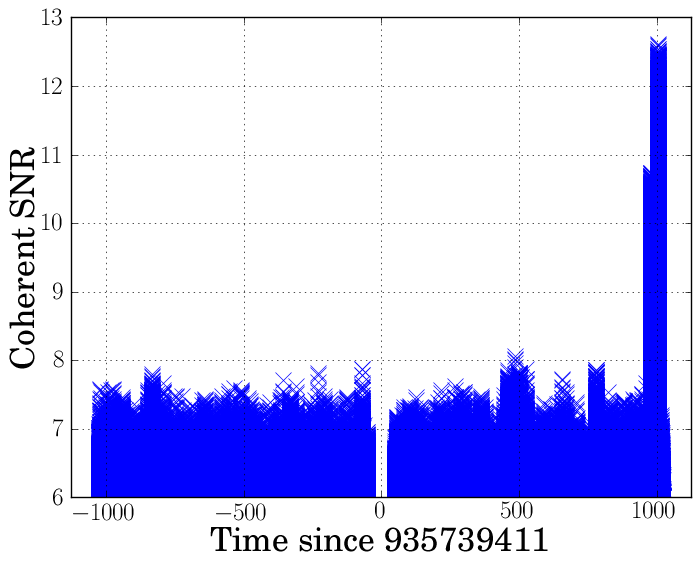
\includegraphics[scale=0.45]{Images/cohSNR.png}
\caption{The coherent SNR time series.}
\label{cohnull}
\end{figure}

\paragraph{Coherent SNR}
The coherent analysis uses the same data generation and matched--filtering procedures as the coincident analysis (already described for GRB070429B): 2190s of GW data was analyzed using H1 and V1 data. The coherent SNR is constructed from equation (\ref{eq:fstat_plus_cross}), from single detector SNR complex series, appropriately shifted and phased. In the analysis, the pipeline generates a trigger at any time for which the coherent SNR threshold is $\rho > 6$. Trigger clustering is done by only keeping the loudest trigger in each 0.1 s time interval.

\paragraph{Null--stream}
The null--stream is a powerful coherent--specific method of identifying and discarding noise transients that a coincident search would normally keep as possible signals. Since coherent SNR can be seen as a projection of coincident SNR on four components, the null--stream can be interpreted as the remainder of the coincident SNR that will not be projected and describes the noise, therefore we can write the null--stream statistic as the difference in quadrature of the coherent and coincident SNR:
%
\begin{equation}
\rho_{\mathrm{N}} = \sqrt{\rho_{\mathrm{coh}}^2 - \rho_{\mathrm{coinc}}^2}
\end{equation}
%
Given a coherent search that looks for signals in the $F_+$ and $F_{\cross}$ polarization channels, the null--stream is the third power channel that will be populated with noise--only transients. Ideally, a gravitational wave signal matching a template will provide no contribution to the null--stream and will be found only in either of the two other channels, so we expect that, for signals, the null--stream statistic will be $\chi^{2}$ distributed with $(2I - 4)$ degrees of freedom, with $I$ the number of detectors used for the search. A noise transient, on the other hand, that is incoherent across the data streams, may give a large coherent \ac{SNR}, but it is also likely to give a large null--stream statistic.

In the analysis, it is required that all events have an \ac{SNR} above 4 in the two most sensitive detectors in the network and the null--stream cut discards any event that has a null--stream statistic larger than $\rho_{\mathrm{N}} > 5.25$. Null streams are generated for analyses using data available from three or more GW detectors; in the case of our GRB, data from only two detectors was used, therefore no null stream was constructed.

\paragraph{Coherent $\chi^2$ test}
The main challenge to constructing a working coherent $\chi^2$ test is to choose the set of template waveforms $T^i$ to replicate the effect of glitches in the \ac{GW} data streams (see Chapter \ref{Chapter Three} and \cite{Harry:2011qh}). These are constructed by taking into account three factors: the waveform is accurate to a certain degree of precision, since the Post--Newtonian (PN) waveforms are derived from Taylor expansions that stop at a certain order \cite{Bliving} and the numerical waveforms suffer from similar inaccuracies \cite{Hannam:2009hh}; the template bank allows for some mismatch between the templates and any potential signal within the full parameter space to a maximal loss in SNR of 3\% \cite{OwenSathyaprakash98}; there are uncertainties in instrumental calibration \cite{Abadie:2010px} which will affect the match between signal and template.

We have described the theoretical framework for the single--detector $\chi^2$ test and application of the test to an analysis. For the multiple--detector test framework we invite the reader to consult \cite{Harry:2011qh}. A figure of the application of the $\chi^2$ test in reducing the numbers of background and injection triggers for GRB090831A can be found in Figure \ref{cohchi}.
%
\begin{figure}[ht]
\centering
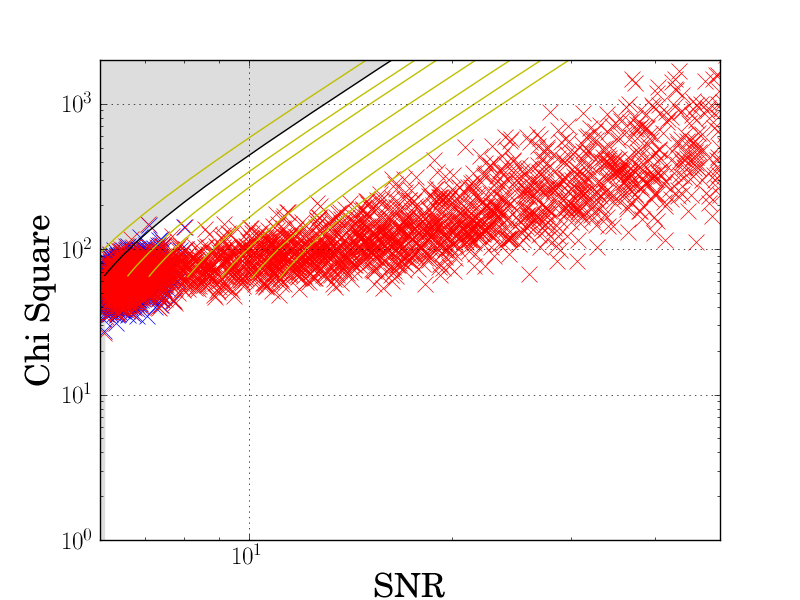
\includegraphics[scale=0.45]{Images/cohChi.png}
\caption{Coherent $\chi^2$ test applied to background (blue) and injection (red) triggers for the analysis of GRB090831A. The cut proves effective in eliminating about a quarter of the lower--SNR background triggers (SNR$\approx$6--7) and a few injections.}
\label{cohchi}
\end{figure}

\paragraph{Coherent bank $\chi^2$ test}
The coherent bank $\chi^2$ test has been conceived and implemented to test the consistency of the recovered SNR from a trigger across the waveform template bank. A \ac{GW} signal will match a certain number of templates giving a pre--described distribution of the SNR in the bank, whereas a glitch would produce numerous high--SNR events randomly distributed in the bank. The coherent bank $\chi^2$ test is calculated in the same manner as the regular $\chi^2$ test but instead it uses a fixed set of $N$ \ac{CBC} template waveforms $T^i$ which remain the same for every template $h(t)$ in the search template bank. These templates are taken from different points across the mass space and are well distributed across it.

For the bank $\chi^{2}$ to be efficient, glitches in the data must have a good overlap with a reasonable fraction of the templates $T^{i}$. While, in general, it is difficult to predict the composition of glitches in the data, it seems reasonable to assume that glitches which produce a large \ac{SNR} for the template $h(t)$ will also have a good overlap with other waveforms in the template space.  Thus, the set of templates which is spread across the parameter space is suitable. For further reference we ask the reader to consult \cite{Hanna:2008} and \cite{Harry:2011qh}.

An example of the application of the coherent bank $\chi^2$ test is shown in Figure ~\ref{cohbank} in the case of GRB090831A analysis.
%
\begin{figure}[ht]
\centering
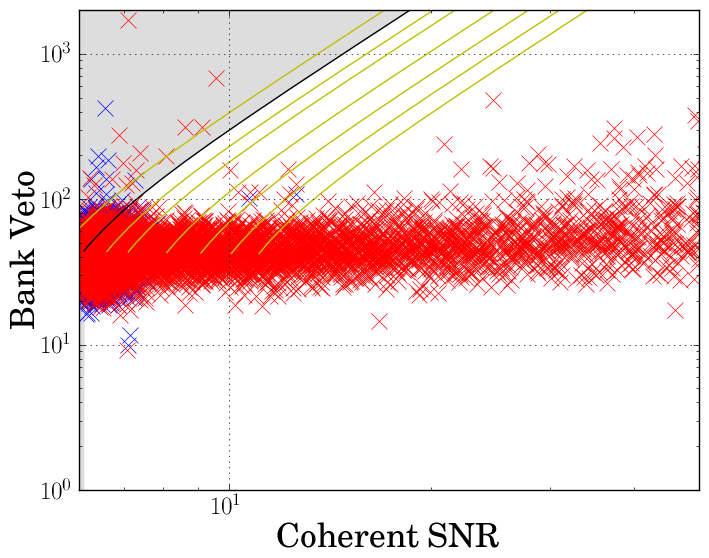
\includegraphics[scale=0.45]{Images/cohBank.png}
\caption{An example of the application of the coherent bank $\chi^2$ test is shown in the case of the GRB090831A analysis. We can see that this discriminator is powerful in this case, in removing background triggers (blue crosses) and a few low--SNR injections (red crosses). There is a number of background triggers close to threshold SNR that the test removes and a glitch at SNR$\approx$7 coincident with an injection, that the test misses.}
\label{cohbank}
\end{figure}
%

\paragraph{Coherent autocorrelation $\chi^2$ test}
Matched--filtering \ac{GW} detector data would produce SNR peaks for both real signals and glitches. The characteristics of a real signal time--series SNR peak differ from those of a glitch. The ``auto'' $\chi^{2}$ test was designed to test the consistency of the \ac{SNR} peak and was initially described in \cite{Hanna:2008}.  It is a similar test to the bank $\chi^{2}$, but if the bank $\chi^{2}$ investigates consistency in \ac{SNR} across the mass space, the auto $\chi^{2}$ tests for consistency of the \ac{SNR} time series.  The test uses the same search template bank containing waveforms $h(t)$ but applies a unique time difference $\Delta t$ of order of the template auto--correlation time , usually $<$0.01 s. Figure ~\ref{cohauto} shows the performance of the autocorrelation $\chi^2$ test in the case of the analysis of GRB090831A. Again, for further reference we ask the reader to consult \cite{Hanna:2008} and \cite{Harry:2011qh}.
%
\begin{figure}[ht]
\centering
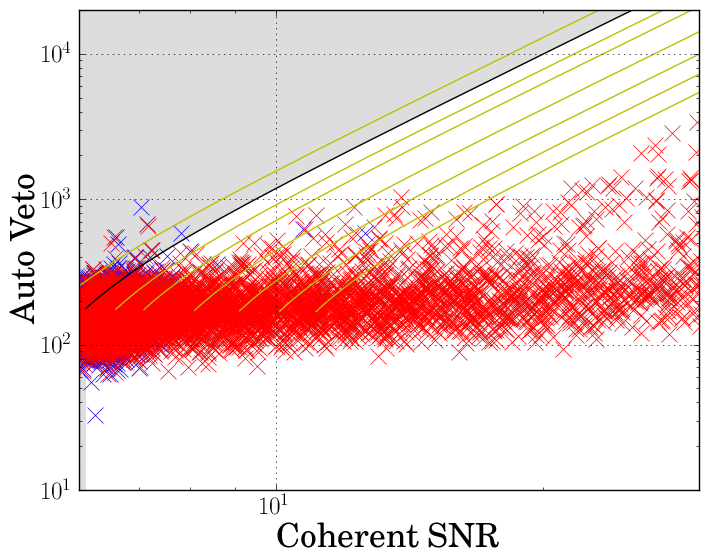
\includegraphics[scale=0.45]{Images/cohAuto.png}
\caption{The autocorrelation $\chi^2$ test for GRB090831A.}
\label{cohauto}
\end{figure}

\paragraph{Coherent background estimation}
After producing a coherent SNR time--series and applying the signal--based vetoes, described above, the analysis will rank the remaining triggers using a detection statistic constructed by using both the null--stream statistic $\rho_{\mathrm{N}}$ and the $\chi^2$ values for each trigger. This ranking statistic, defined as $\rho_{det}$ and given by
%
\begin{equation}\label{eq:rho_det}
\rho_{\mathrm{det}} =  \left\{
\begin{array}{ll}
 \displaystyle \rho_{\mathrm{new}} , & \rho_{N} \le 3.5 \\[0.1in]
 \displaystyle \frac{\rho_{\mathrm{new}}}{\rho_{\mathrm{N}} - 2.5} ,
 & 3.5 < \rho_{N} < 5.25 \, .
\end{array}
\right.
\end{equation}
%
where ``\textit{new SNR}'':
%
\begin{equation}
 \rho_{\mathrm{new}} = \left\{
\begin{array}{cl}
\displaystyle \rho, & \chi^2 \le n_{\mathrm{dof}} \\[0.1in]
\displaystyle \frac{\rho}{\left[\left(1 +
\left(\frac{\chi^2}{n_{\mathrm{dof}}}\right)^{4/3}\right)/2\right]^{1/4}}, & \chi^2 >
n_{\mathrm{dof}}
\end{array}
\right.
\end{equation}
%
where $\rho$ is the matched--filter trigger SNR. This detection statistic has the same expression as the ranking statistic used by the coincident analyses during S6/VSR2 and 3, and is a step forward from the S5/VSR1 effective SNR, with a better glitch rejection power at lower values of the $\chi^2$; $n_{\mathrm{dof}}$ represents the number of degrees of freedom for the $\chi^2$. The detection statistic is weighted by both the null--stream statistic and by the chi--squared values in order to improve the capacity of rejecting non--stationary noise triggers. Figure \ref{cohBG} shows the cumulative number of background events versus detection statistic in the coherent analysis of GRB090831A. By computing the background (off--source) trigger rate, expected purely from detector noise, we are able to assign a false alarm probability (FAP) to a possible detection event in the on--source 6s window. The false alarm probability is computed using the same formalism for the coincident search, and the detection (or non--detection) statement is made by quoting the results of equation:
%
\begin{equation}
\mathrm{FAP} = \frac {N(\rho>\rho_0)}{N_0}
\end{equation}
%
where the fraction is the number of background events with a coherent SNR $\rho$ larger than the onsource $\rho_0$, $N(\rho>\rho_0)$, divided by the effective number of off--source trials, $N_0$.

\begin{figure}[ht]
%\begin{minipage}[b]{0.5\linewidth}
%\centering
%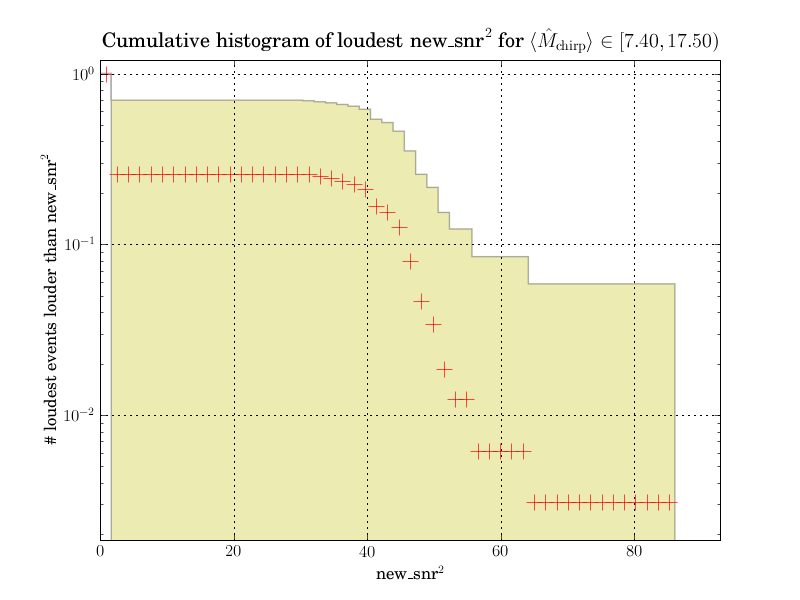
\includegraphics[scale=0.45]{Images/coincBG.png}
%\caption{Coincident analysis loudest background events in the high chirp mass bin. We can find notably more background events than in the coherent analysis of the same data; the maximum value of the detection statistic is $\approx$9.}
%\label{coincBG}
%\end{minipage}
%\hspace{0.5cm}
%\begin{minipage}[b]{0.5\linewidth}
\centering
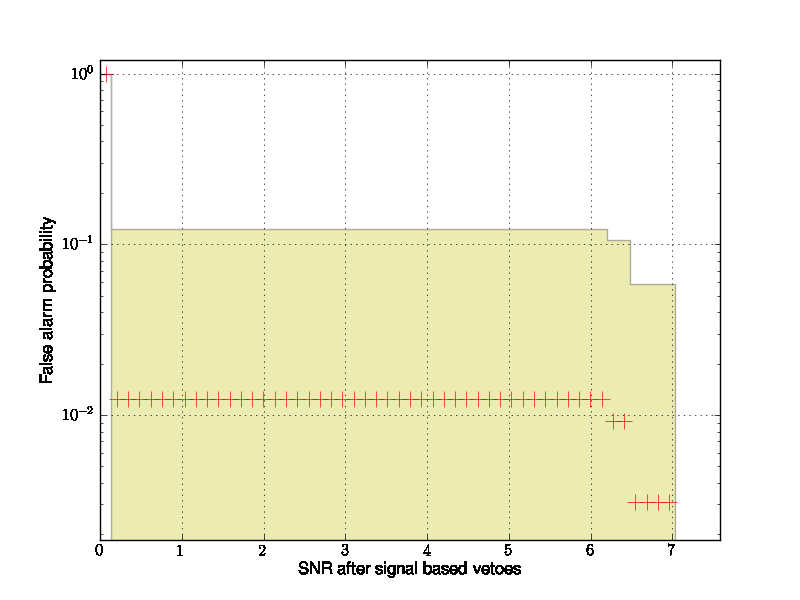
\includegraphics[scale=0.60]{Images/cohBG.png}
\caption{Coherent analysis loudest background events in the high chirp mass bin. We can find very few triggers that pass the signal--based vetoes and the maximum value for the detection statistic is $\approx$7.}
\label{cohBG}
%\end{minipage}
\end{figure}

\paragraph{Results: distance exclusion and search sensitivity}
No detection of a GW signal was made: a single event was found in the on--source in the low chirp mass bin with a FAP=0.71. In the case a GW signal detection is not made in association with the GRB, we would want to draw a set of parameters that characterize the search sensitivity. For each GRB we derive a 90\% confidence lower limit on the distance to the GRB progenitor for either the astrophysically--motivated NS--NS or NS--BH merger models. The method to determine this exclusion distance is further detailed in Chapter \ref{Chapter Seven}, where this is explained in light of the search for GW associated with the short hard GRBs detected by the IPN. Its application is the same here. In short, the 90\% exclusion distance is the distance where the efficiency of recovering injections (number of ``missed'' injections divided by number of ``found'' injections) drops below 90\%; or, it is the distance to which we are 90\% confident there was no CBC event associated with the particular analyzed GRB given the present search parameters (template bank, thresholds, signal--based vetoes, etc.). 

For GRB090831A the exclusion distance for NS--NS was 5 Mpc and for NS--BH, 9 Mpc. As a result of analyzing data around the 26 \emph{Swift} and Fermi--GBM short bursts during S6/VSR23, the median exclusion distance for NS--NS was 17 Mpc and for NS--BH, 29 Mpc \cite{lvc:s6grb}.

\section{Triggered searches: sensitivity improvement}
\label{sens_imprv}

We have presented two searches for GW associated with two short hard gamma-ray bursts; we used the GRB times and sky locations to perform triggered searches at the bursts' times and sky positions. It would be very useful to know how much we are gaining in sensitivity by doing a triggered search limited both in time (more generally, around the interesting electromagnetic transient, e.g., here the short GRB burst times) and in sky location (at the GRB right ascension and declination) as compared to an all--time, all--sky search. In this section we will estimate this increase in sensitivity by looking at different lengths of background data centered around the trigger time of our test GRB090809B and by comparing the background obtained from an untriggered (all--sky) search to the background obtained by performing a search at the sky location of the GRB. This will be just an estimation since to be able to get a decisive figure we will have to look not only at the background distribution but also at the simulations' recovery in the untriggered and triggered situations for multiple GRBs. We leave this for a future work.

To do this, we use the pipeline that searched for \ac{CBC} signals in an all--sky, all--time regime during S6/VSR23 (named ``ihope'', described in \cite{Abadie:2010yb, Colaboration:2011nz}). The pipeline looked for coincident events in each of the detectors that were available for the search and is, in broad lines, the untriggered equivalent of the coincident triggered pipeline described in Chapter \ref{Chapter Four}, Section ~\ref{coincident_GRB}. The reason we use ``ihope'' is that we need data from an untriggered search that is not available using the standard GRB pipeline and we need consistency (the same search method applied for different scenarios) to be able to compare results (just look at SNR values for fixed false alarm rates). The data was analyzed in four ways:

\begin{itemize}
\item
A week of data around the GRB090809B trigger time analyzed in all--sky, all--time regime (GPS 933895709, the analysis was performed between GPS 933379143 and 933984087). A histogram of the loudest background events in the zero--lag and timeslides (100 timeslides) is shown in Figure ~\ref{090809B_allsky_1week}. The ``loudest'' zero--lag event has an SNR$\approx$9.2 and the ``loudest'' timeslide event has an SNR$\approx$10.3. 

\begin{figure}[ht!]
\centering
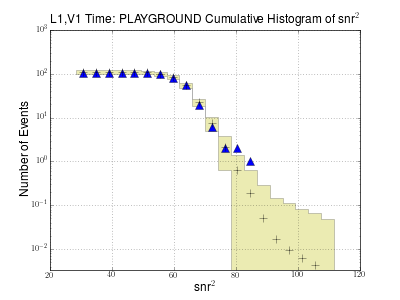
\includegraphics[scale=0.55]{Images/090809B_allsky_1week.png}
\caption{Histogram of the loudest background events in the zero--lag (triangles) and timeslides (100 timeslides, crosses) for a week of data around the GRB090809B trigger time, for an all--sky search. The ``loudest'' zero--lag event has an SNR$\approx$9.2 and the ``loudest'' timeslide event has an SNR$\approx$10.3. The analysis was made using the all--time, all--sky search pipeline (ihope, \cite{Abadie:2010yb, Colaboration:2011nz}).}
\label{090809B_allsky_1week}
\end{figure}

\item
A single day of data around the GRB090809B trigger time analyzed in all--sky, all--time regime (GPS 933895709, the analysis was performed between GPS 933852509 and 933938909). A histogram of the loudest background events in the zero--lag and timeslides (100 timeslides) is shown in Figure ~\ref{090809B_allsky_1day}. The ``loudest'' zero--lag event has an SNR$\approx$8.4 and the ``loudest'' timeslide event has an SNR$\approx$9.5.

\begin{figure}[ht!]
\centering
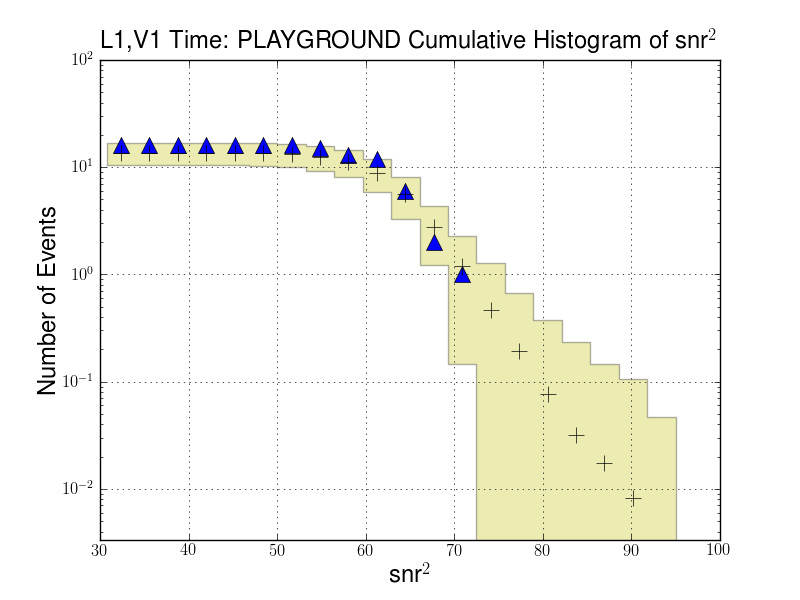
\includegraphics[scale=0.55]{Images/090809B_allsky_1day.png}
\caption{Histogram of the loudest background events in the zero--lag (triangles) and timeslides (100 timeslides, crosses) for a day of data around the GRB090809B trigger time, for an all--sky search. The ``loudest'' zero--lag event has an SNR$\approx$8.4 and the ``loudest'' timeslide event has an SNR$\approx$9.5. The analysis was made using the all--time, all--sky search pipeline (ihope, \cite{Abadie:2010yb, Colaboration:2011nz}).}
\label{090809B_allsky_1day}
\end{figure}

\item
2000 s of data around the GRB090809B trigger time analyzed in all--sky, all--time regime (GPS 933895709, the analysis was performed between GPS 933894709 and 933896709). A histogram of the loudest background events in the zero--lag and timeslides (100 timeslides) is shown in Figure ~\ref{090809B_allsky_2000s}. The ``loudest'' zero--lag event has an SNR$\approx$8.4 and the ``loudest'' timeslide event has an SNR$\approx$9.2.

\begin{figure}[ht!]
\centering
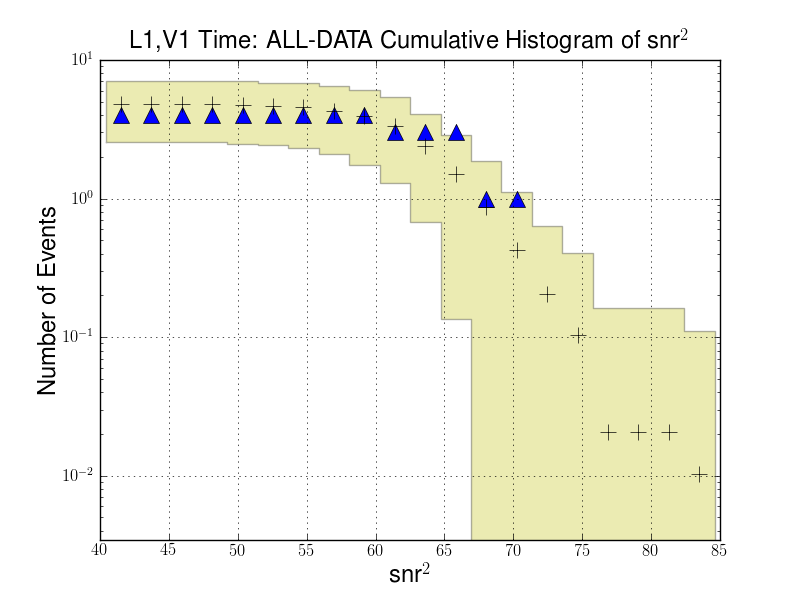
\includegraphics[scale=0.55]{Images/090809B_allsky_2000s.png}
\caption{Histogram of the loudest background events in the zero--lag (triangles) and timeslides (100 timeslides, crosses) for 2000 s of data around the GRB090809B trigger time, for an all--sky search. The ``loudest'' zero--lag event has an SNR$\approx$8.4 and the ``loudest'' timeslide event has an SNR$\approx$9.2. The analysis was made using the all--time, all--sky search pipeline (ihope, \cite{Abadie:2010yb, Colaboration:2011nz}) on a limited size data stretch.}
\label{090809B_allsky_2000s}
\end{figure}

\item
2000 s of data around the GRB090809B trigger time analyzed in triggered regime (GPS 933895709, the analysis was performed between GPS 933894709 and 933896709). A histogram of the loudest background events in the zero--lag and timeslides (100 timeslides) is shown in Figure ~\ref{090809B_directed_2000s}. The ``loudest'' zero--lag event has an SNR$\approx$7.9 and the ``loudest'' timeslide event has an SNR$\approx$8.6. The analysis was made by imposing condition on timedelays between operational detectors to search the the GRB sky location.

\begin{figure}[ht!]
\centering
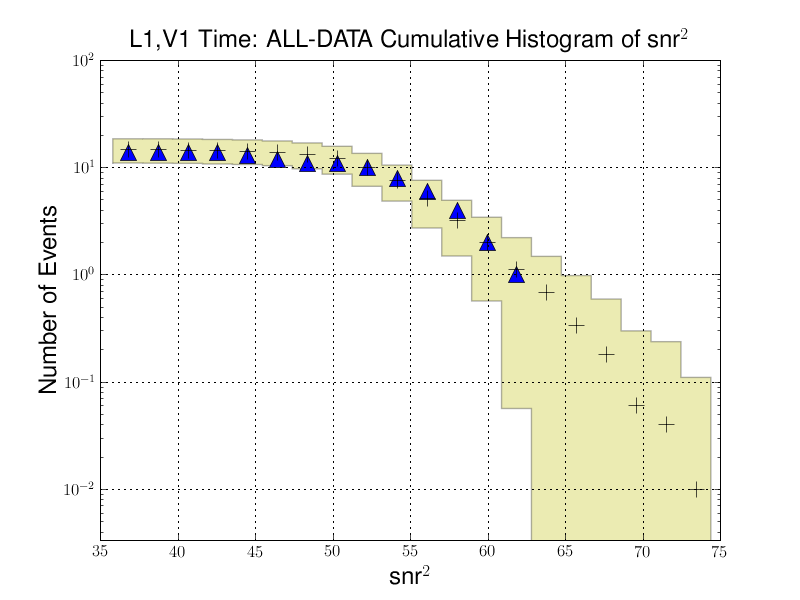
\includegraphics[scale=0.55]{Images/090809B_directed_2000s.png}
\caption{Histogram of the loudest background events in the zero--lag (triangles) and timeslides (100 timeslides, crosses) for 2000 s of data around the GRB090809B trigger time, for a triggered search at the sky location of the GRB. The ``loudest'' zero--lag event has an SNR$\approx$7.9 and the ``loudest'' timeslide event has an SNR$\approx$8.6. The analysis was made using the all--time, all--sky search pipeline (ihope, \cite{Abadie:2010yb, Colaboration:2011nz}) on a limited size data stretch imposing condition on timedelays between operational detectors to search the the GRB sky location.}
\label{090809B_directed_2000s}
\end{figure}

\end{itemize}

Suppose the data does not contain ``excessively loud'' glitches (previously removed by signal--based vetoes), and considering that the maximum SNR $\rho_{max}$ of the loudest event from the timeslid data (since a reliable background estimation can be done with timeslides only) at a fixed FAP and for the same search configuration in each of the cases above, characterizes the sensitivity of the search. The maximum SNR is a measure of how far in terms of distance can the search detect CBC events, relating to distance $\rho_{max} \propto 1/D_{max}$. We can estimate an increase of 13\% in sensitivity distance when reducing the analysis time from a week to 2000 s and another 7\% when using the sky location of the GRB for a triggered search. This amounts to approximately 20\% increase in sensitivity (distance) when comparing a week of analyzed data in all--time, all--sky regime with 2000 s of analyzed data in triggered regime on sky location. If we look at Figures \ref{090809B_allsky_1week} and \ref{090809B_allsky_1day} we notice that an event with effective SNR 90 will have a decrease in false alarm probability of order $7 \times 10^{-2}$ when shortening the analysis time from a week to a day, so roughly a measure of $10^{-2}$ FAP drop per day.

The 20\% increase in distance sensitivity translates into $\approx$73\% increase in volume sensitivity, which, in turn, assuming a naive constant number density for short GRBs, increases by $\approx$73\% the number of observable bursts.

These results are summarized in Table \ref{trig_untrig_comp}. Knowing the sky location of the GRB accounts for an increase of $\approx$7\% whereas knowing the exact time and being able to perform a search on a short stretch of data, without using a privileged sky location, increases the sensitivity by $\approx$13\% (1 week $\rightarrow$ 2000s), this shows that the major contribution to sensitivity increase from a triggered (time and sky location) search is knowing the exact trigger time. 

This estimation was performed using coincident data from \emph{two} GW detectors -- in the case of a triggered search using three or more detectors the sky localization will be improved (see Chapter \ref{Chapter One} for reference) therefore, the search sensitivity will increase as compared to the all--sky search. Further in--depth studies are needed, especially with the commissioning of Advanced LIGO, with trigger rates that are yet to be measured.

\begin{table}[ht!]
 \begin{tabular}{|l|l|l|l|l|}
 \hline
 \hline
 Case & FAP & $\rho_{max}$ & $D \propto 1/\rho_{max}$ & Sens. Increase (\%) \\
 \hline
 1 week ALL-SKY & $10^{-2}$ & 10.300 & 0.097 & n/a \\
 1 day ALL-SKY & $10^{-2}$ & 9.486 & 0.105 & 8\% \\
 2000s ALL-SKY & $10^{-2}$ & 9.110 & 0.110 & 4.8\% \\
 2000s TRIGGERED & $10^{-2}$ & 8.544 & 0.117 & 6.4\% \\
 \hline
 \hline
 \end{tabular} 
 \caption{Relative increases in search sensitivity for an identical search (same search parameters, using a single GRB trigger) performed on 1 week, 1 day and 2000s of data in all--sky mode and 2000s of data in typical GRB--triggered mode. $\rho{max}$ results are quoted at a fixed false alarm rate. Results suggest a typical increase of $\approx$20\% in sensitivity from a search on 1 week of data all--sky to 2000s triggered; knowing the sky location of the GRB accounts for an increase of 6.4\% whereas knowing the exact time and being able to perform a search on a short stretch of data increases the sensitivity by 12.8\% (1 week $\rightarrow$ 2000s).}
 \label{trig_untrig_comp}
\end{table}

\section{Discussion}

We have presented two different analysis methods to search for compact binary coalescences around short hard GRB triggers. Both methods have been used to produce results and publications: the coincident method was used in association with short GRB triggers during S5/VSR1 \cite{Abadie:2010uf} and the coherent method was used in association with short GRBs during S6/VSR2 and 3 \cite{lvc:s6grb}. Both methods make use of the sky location and time of the GRB event to gain search sensitivity as compared to all--time, all--sky searches. Both methods use matched--filtering the GW data through a set of theoretical waveforms (the ``template bank'') at their core, but the fundamental way of combining the data from multiple GW detectors differs. Whereas the coincident method looks for outstanding events that should be present in multiple detectors in the same time--chirp--mass window, the coherent method combines \emph{all} the data from \emph{all} the available GW detectors to extract two possible types of channels, a GW data channel and multiple noise channels (null streams). This, combined with a series of very strong signal--based veto tests, make the coherent search a more sensitive one compared to the coincident search.

We have presented search results from the coincident analysis associated with the \emph{Swift}--detected GRB070429B and coherent analysis associated with the Fermi--GBM--detected GRB090831A. No gravitational waves were detected in the 6s on--source window of any of these two short bursts. Therefore, we have computed a 90\% confidence distance to the GRB progenitor for the two predicted emission models (NS--NS or NS--BH).

We have also estimated the increase in sensitivity gained from performing a triggered search compared to an all--sky, all--time search. The sensitivity increase comes from both knowing the sky location and the time of the astrophysical trigger we wish to follow--up in GW data. This was done by successively comparing GW analyses that used data of different lengths and were performed either in all--sky or in triggered modes. W found an estimated 20\% sensitivity increase.

There still are ways to improve the current triggered search. One possibility would be an optimal choice for the detection statistic thresholds; another one would be better astrophysically--motivated priors on inclination or distance to the source.

This chapter was meant as a brief introduction to both coincident and coherent analysis methods and by no means as an in--depth study. For further reference to applying the coincident method to GRB triggered searches we invite the reader to consult \cite{Abadie:2010uf}; for the coherent application we point the reader to \cite{Harry:2010fr} and references therein.
